\chapter{\cc{逻辑}{Logic}}

\begin{flushright}
	\english{The only way to rectify our reasonings is to make them as tangible as those of the Mathematicians, so that we can find our error at a glance, and when there are disputes among persons, we can simply say: Let us calculate [calculemus], without further ado, to see who is right.}\\ --- Leibniz
\end{flushright}
\minitoc

	\section{\cc{人脑思考的三大模式}{The 3 main modes of human thinking}}

		\subsection{Deduction}
		\subsection{Abduction}
		\subsection{Induction}

	\section{\cc{命题逻辑}{Propositional logic}}
	
		\subsection{Boolean algebra}

假设大家都熟悉 Boolean algebra,一个比较抽象的定义是:  a Boolean algebra is a \textbf{complemented distributive lattice}.

The Boolean algebra with $2^4$ elements:
\begin{equation}
\vcenter{\hbox{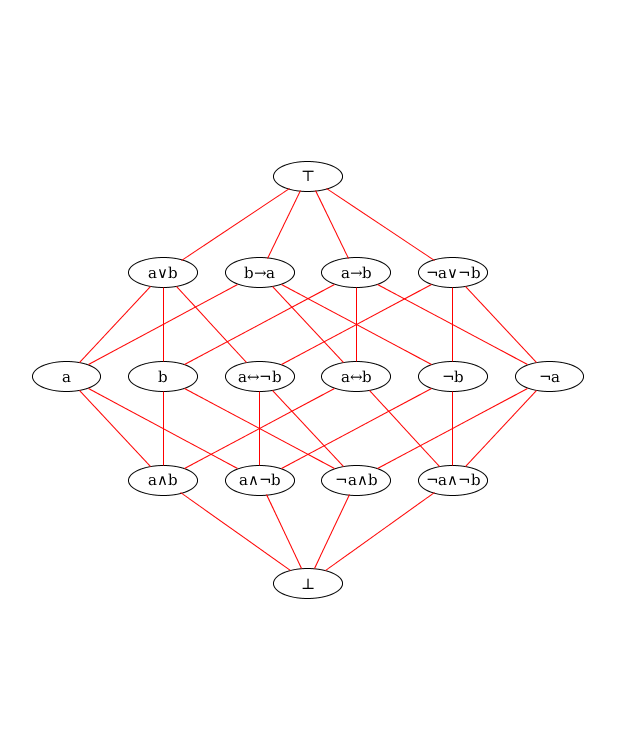
\includegraphics[scale=0.6]{Boolean-algebra-2xx4.png}}}
\end{equation}
其中 $a \rightarrow b \equiv \neg a \vee b$, $b \rightarrow a \equiv a \vee \neg b$。

		\subsection{Boolean lattice}

\begin{eqnarray}
a \rightarrow b = \top & \Leftrightarrow & \neg a \vee b = \top \nonumber \\
 & \Leftrightarrow & a \vee b = a \nonumber \\
 & \Leftrightarrow & a \leq b \quad \quad \text{(by definition of lattice)}
\end{eqnarray}
所以 $a \leq b$ 定义了一个 order relation,这就是 the Boolean lattice associated with the Boolean algebra,两者是等价的。 

这是包含两个命题的 Boolean lattice(但似乎不是 complete atomic Boolean lattice):
\begin{equation}
\vcenter{\hbox{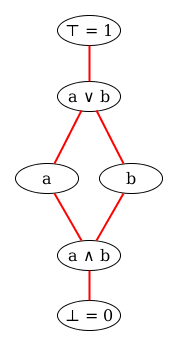
\includegraphics[scale=0.6]{Boolean-lattice.png}}}
\end{equation}

对於 任意 $a$ 恒有:
\begin{eqnarray}
\bot \leq & a & \leq \top \nonumber \\
\bot \rightarrow & a & \rightarrow \top
\end{eqnarray}
\begin{tabbing}
\hspace*{2cm}\=  \kill
因为: \> 由假的前提 ($\bot$) 可以推出任意结论 (\english{ex falso sequitur quodlibet}),\\
      \> 而由任意前提都可以推出 恒真命题 ($\top$)。\\
\end{tabbing}

$a \rightarrow b \Leftrightarrow a \leq b$ 但方向相反,原因是 $0 \leq 1$,在 lattice 中越往下的命题 越难满足。

		\subsection{Knowledge and lattice structure}

如何用 lattice 表达 AI 中的逻辑结构?  似乎有两个方法。  首先,将所有可能出现的命题集合都表达成 lattice 中的某些节点:		
\begin{equation}
\vcenter{\hbox{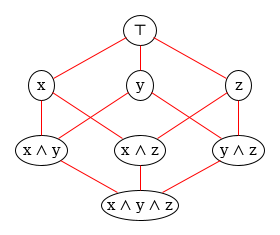
\includegraphics[scale=0.7]{Boolean-lattice-eg1.png}}}
\label{regular knowledge lattice}
\end{equation}
换句话说,lattice 中每个节点 表示 mental state 的一个 \textbf{状态}。  进行逻辑思考时,由一个状态跳到另一个状态,这 transition function 就是 $F$(亦即我提议用 神经网络 模拟的函数)。  换句话说,lattice 代表 \textbf{状态空间},但 \textbf{知识} 是储存在 $F$ 里面。 所谓 \textbf{知识} 其实就是这样的一些 逻辑 \textbf{rules}(或者叫 \textbf{conditionals}):
\begin{eqnarray}
& p \rightarrow q & \\
\nonumber {\raisebox{5pt}{\mbox{例如}}} &\begin{tikzpicture}
% \usetikzlibrary{arrows}
\usetikzlibrary{shapes}
% \tikzstyle{every node}=[draw=black, ellipse, minimum width=50pt, align=center]
\node[left=35pt, draw, shape=rounded rectangle] (a) {吃了不洁食物};
\node[draw, shape=rounded rectangle] (b) {肚痛};
\draw[thick] (a) edge[->] (b);
\end{tikzpicture}&
\end{eqnarray}
在上例中(fig. \ref{regular knowledge lattice}),状态空间 包含所有可能的命题组合,可以说这个 lattice 是 ``regular'' 的(但这 terminology 可能不正确)。 

如果在 lattice 中加入一些已知的 knowledge,例如 $y \rightarrow x$,则某些 节点 会消失,而且加入了一个新的 edge: 
\begin{equation}
\vcenter{\hbox{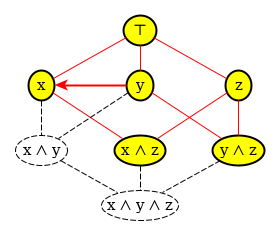
\includegraphics[scale=0.7]{Boolean-lattice-eg1b.png}}}
\quad \quad = \quad \quad
\vcenter{\hbox{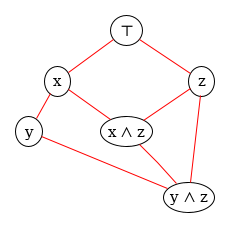
\includegraphics[scale=0.7]{Boolean-lattice-eg2.png}}}
\end{equation}
这时,状态 lattice 变得 ``irregular'',但 $F$ 只需在这 lattice 中容许的节点上移动。

		\subsection{Heyting algebra}

\underconst

		\subsection{Boolean ring}

给定一个 Boolean algebra,可以定义:
\begin{eqnarray}
\boxed{symmetric difference} \quad a + b &=& (a \wedge \neg b) \vee (\neg a \wedge b) \nonumber \\
a \cdot b &=& a \wedge b
\end{eqnarray}
则 $(A, +, \cdot)$ 构成一个 Boolean ring。  

\begin{flalign}
a + a = 0 &&
\end{flalign}
所以 Boolean ring 的 characteristic 是 2。

在 Boolean ring 里,complement 可以这样表示:
\begin{equation}
\neg a = a + 1
\end{equation}

(在数学上,据说 ring 较方便研究,但我暂时不知其细节。)

		\subsection{Ideals and filters}

Ideal 的概念来自 algebraic geometry。  如果我们有一组代数方程:
\begin{eqnarray}
f_1 &=& 0, \nonumber \\
 &\vdots& \nonumber \\
f_s &=& 0
\end{eqnarray}
则由 $f_s$ 组成的 线性组合 也会是这组方程的解:
\begin{equation}
h_1 f_1 + h_2 f_2 + ... + h_s f_s = 0.
\end{equation}
形如左边那种元素,就是这 ideal 的元素。  The ideal generated by $f_s$,记作 $\langle f_1, ... , f_s \rangle$,它可以看成是方程组 $f_1 = f_2 = ... = f_s = 0$ 的「多项式后果」 (\textbf{polynomial consequences}) 的全体集合。 \parencite{Cox2007} p.31.

在逻辑上,\uline{ideal 对应於一些 逻辑式子 的 consequences},但由於在 代数几何 中,ideal 的定义是 algebraic equations = 0,但逻辑 中 真 = 1,所以需要 ideal 的 dual concept,即 \textbf{filter}。

在 Boolean algebra 中,如果问「某一命题 $q$ 是不是前提 $\Gamma$ 的结论?」其答案等於问: $q$ 是不是属於由 $\Gamma$ 生成的 \textbf{ideal} 之中? 在 computational algebraic geometry 中,ideal membership 的问题可以用 \textbf{Gr\"{o}bner basis} 的方法解答。 暂时我不清楚这个方向有没有优势。

我觉得现时一个重要问题是: \unline{如果我们用 神经网络 $\,F$ 近似地}\textbf{\unline{ 模拟}}\unline{ 逻辑 $\; \vdash$,而逻辑有其 代数结构,则这代数结构 如何 影响 $\,F$ 的结构,及 $\,F$ 的 learning algorithm}?  这问题会在 \S\ref{Logic and NN} 考虑。

\subsection{人工智能中的 forward chaining}




	\section{\cc{谓词逻辑/一阶逻辑}{Predicate logic / first-order logic}}
	
	\section{\cc{逻辑推理算法}{Inference (classical)}}
	
		\subsection{\cc{消解算法 (resolution)}{Resolution algorithm}}
		\subsection{\cc{同一化算法 (unification)}{Unification algorithm}}
	
	\section{\cc{二阶逻辑/高阶逻辑}{Second-order / higher-order logic}}

	\section{\cc{$\lambda$-演算,组合逻辑}{$\lambda$-calculus, combinatory logic}}

	\section{\cc{各种逻辑结构之间的关系}{Relations between various logical structures}}

\begin{equation}
\vcenter{\hbox{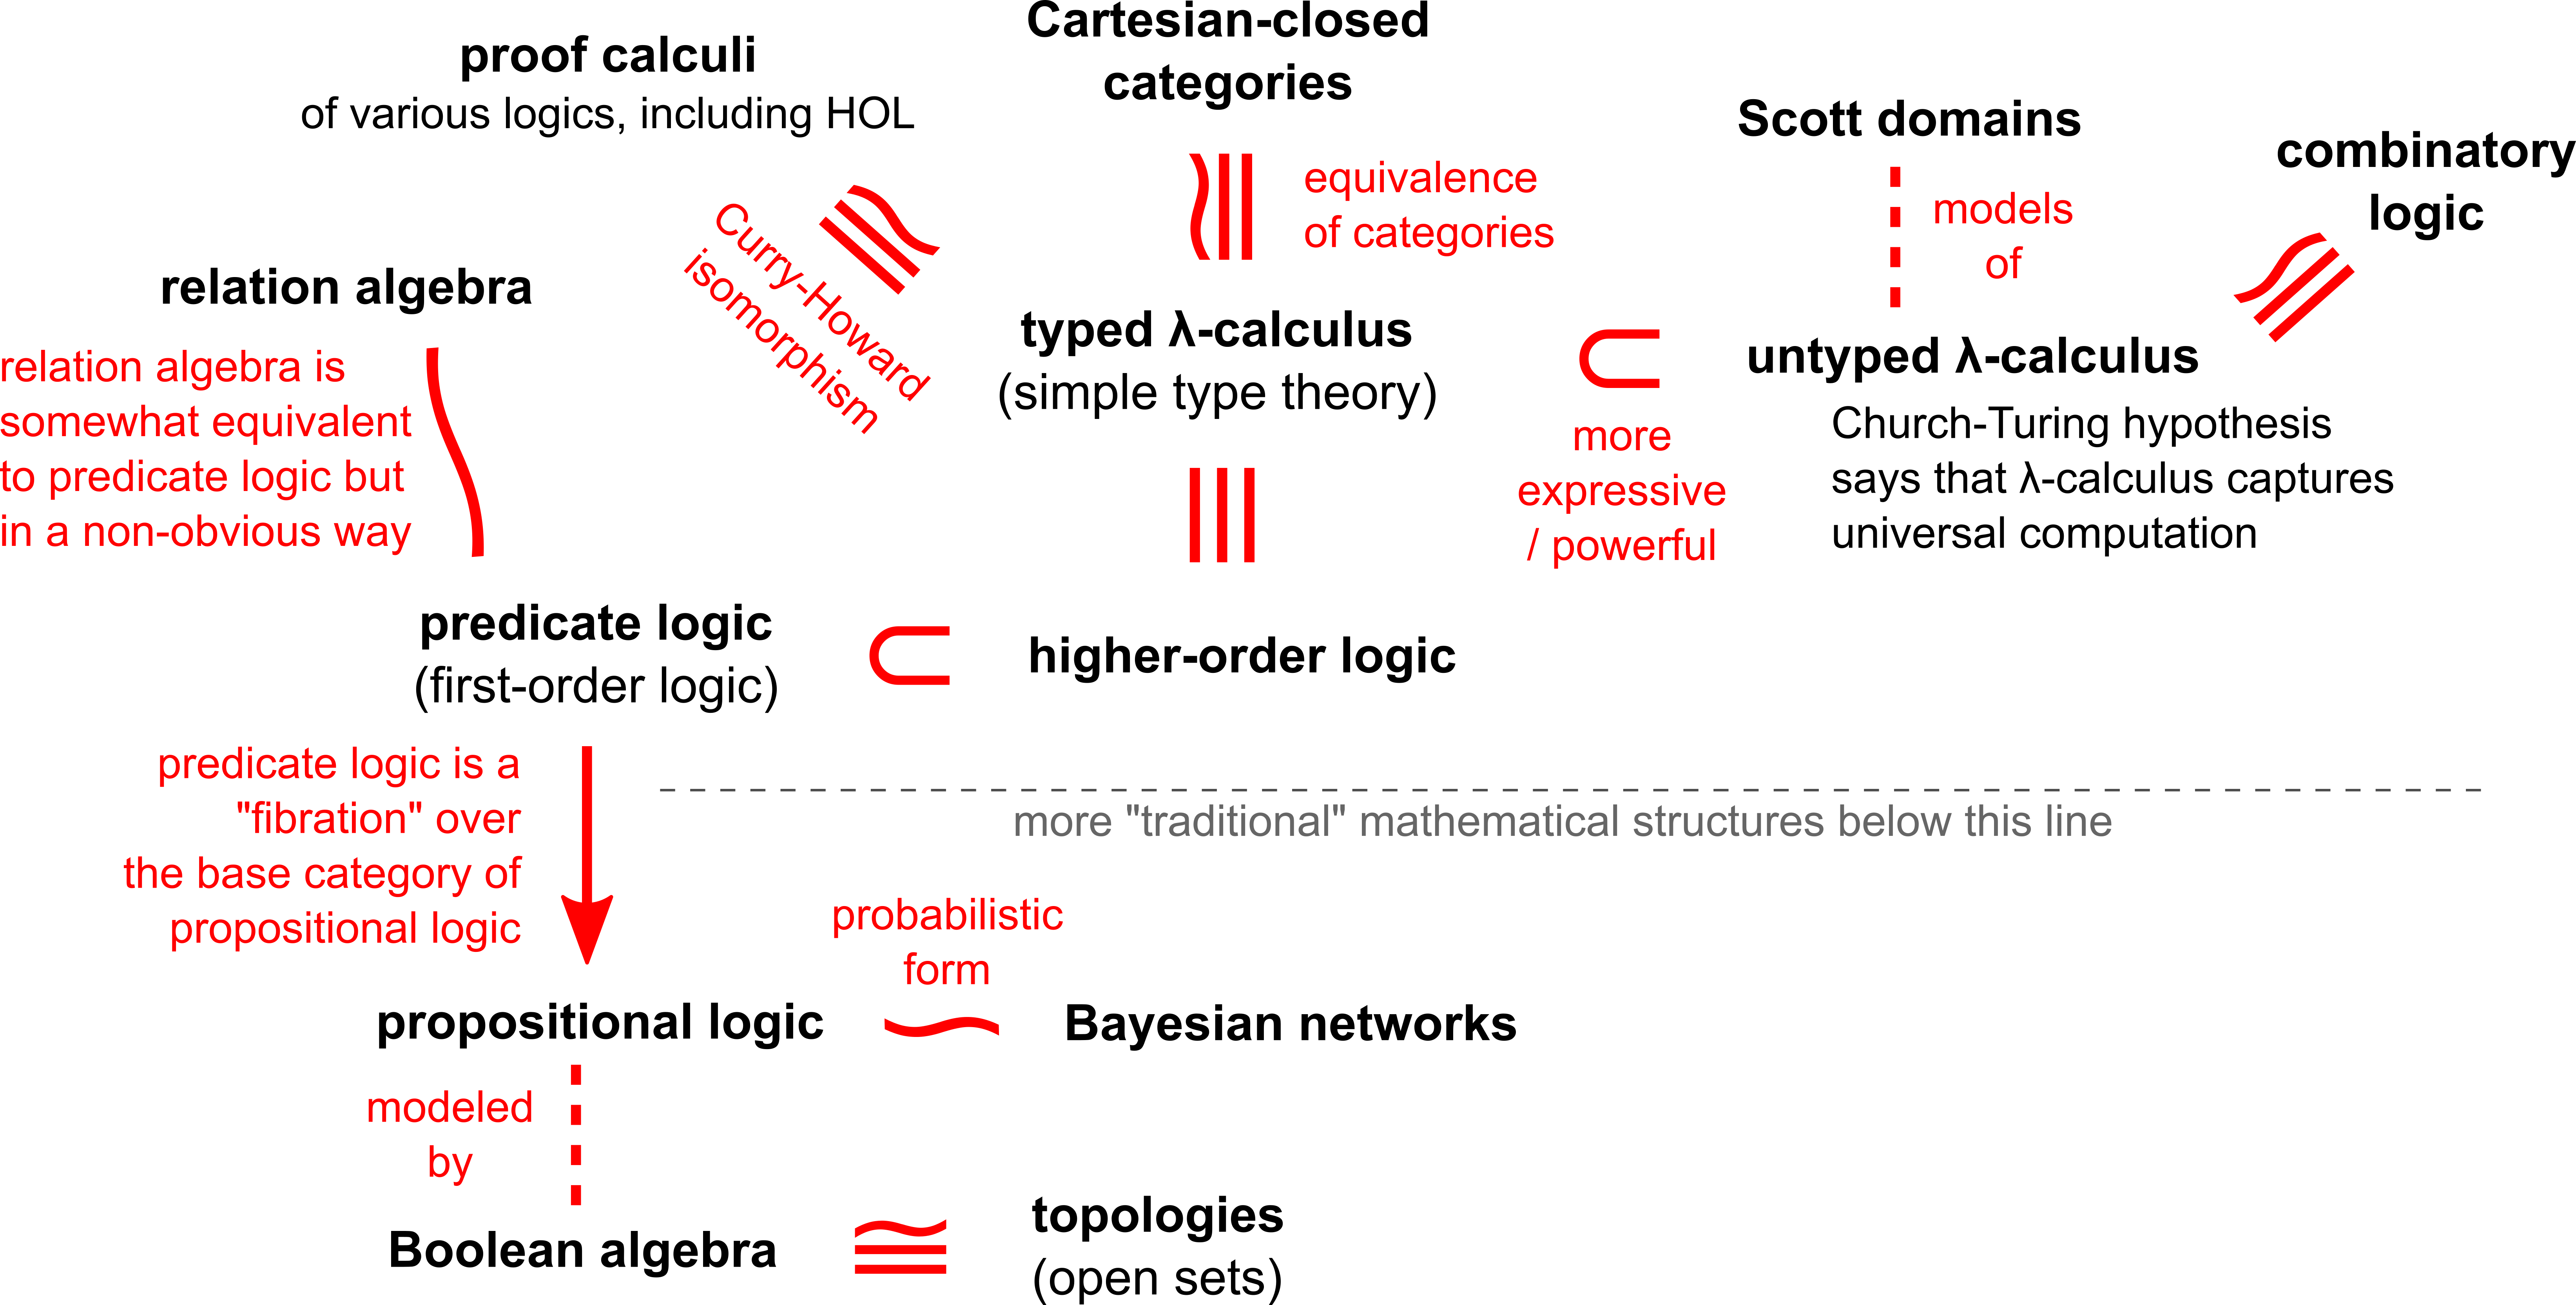
\includegraphics[scale=0.7]{world-of-logical-structures.png}}}
\end{equation}

在上图中最「麻烦」的似乎是 由 propositional logic 提升到 predicate logic 的 \textbf{fibration}。 从命题逻辑上升到 type theory 可以透过 Curry-Howard isomorphism(下节介绍);  在这过程中,propositions 对应 \textbf{types},predicates 对应 \textbf{dependent types}。

举例来说:
\begin{eqnarray}
\boxed{命题}  \quad & \mbox{『约翰是男人』} & \quad \formula{Male(john)} \nonumber \\
\boxed{命题}  \quad & \mbox{『约翰爱玛莉』} & \quad \formula{Loves(john, mary)} 
\end{eqnarray}
Predicate 是一种函数,它吃一些 objects,吐出一个 proposition。

在 type theory 那边,dependent type 吃一些 terms,吐出一个 type。 例如 $\formula{ARRAY}(n)$ 是一个 dependent type,它吃掉一个整数 $n$,吐出一个长度为 $n$ 的 $\formula{ARRAY}$ type。 

两边之间有这样的 Curry-Howard 对应:
\begin{eqnarray}
\mbox{\textbf{Logic}} &  & \mbox{\textbf{Type theory}} \nonumber \\
\mbox{formulas} & \leftrightsquigarrow & \mbox{types} \nonumber \\
\mbox{proofs} & \leftrightsquigarrow & \mbox{terms} \nonumber \\
\mbox{predicates} & \leftrightsquigarrow & \mbox{dependent type: terms $\rightarrow$ type}
\end{eqnarray}
Dependent type 是一个吃 terms 吐出 type 的函数。  它对应於逻辑 predicate,换句话说,predicate 是一个吃 proofs 吐出 proposition 的东西。  这有点奇怪,因为 predicate 通常吃的是逻辑里的 objects(也可以叫做 logic constants)。  但细想一下,如果 $\formula{john}$ 存在於 $\formula{Male}$ 这个集合内,则 $\formula{john}$ 顺理成章地可以看成是 $\formula{Male(john)}$ 此一命题的 proof。 换句话说,逻辑 objects 可以看成是逻辑上的 proofs。

Simple type theory 与 CCC 有 equivalence of categories(在 \parencite{Lambek1986} 书中有论述); 在这 等价关系中,types 对应於 morphisms(例如 morphism $f: A \rightarrow B$ 对应於 $x: A \vdash f(x): B$)。 换句话说,似乎要模拟 predicate logic 的关键是需要某些 ``morphisms''。

注意: simple type theory 亦被叫作 higher-order logic,它是 first-order logic 的扩充,但这扩充并不需要经过 Curry-Howard isomorphism,因此往往造成混淆。  现代逻辑的研究似乎特别关注 Curry-Howard 同构。

% Type constructor 是指任何输出是 ``type'' 的函数。 

	\section{\cc{Curry-Howard 同构}{Curry-Howard isomorphism}}

$\lambda$-calculus 是一切「计算」(computable functions) 的形式。  Type theory 的作用是 enforce type discipline 以避免一些 paradox,例如 untyped $\lambda$-calculus 里面有 Curry paradox。

在 proof theory 里面,逻辑的 \textbf{后设法则} (meta-logical rules) 描述怎样由一些 逻辑式子 推导 到另一些 式子。 由 Brouwer-Heyting-Kolmogorov 提出的想法是: 将 \textbf{逻辑蕴涵} (implication) 看成是一些 functions 或 mappings。 这个想法再经 Curry-Howard 进一步发展,认为 proofs 就是「计算」,所以对应於 $\lambda$-terms。 
\begin{eqnarray}
\textbf{Type theory}                              &      & \textbf{Logic} \nonumber \\
\mbox{(``programs'')} \quad \lambda\mbox{-terms}  & \sim & \mbox{proofs} \nonumber \\
\mbox{types}                                      & \sim & \mbox{propositions}
\end{eqnarray}

详细可参看 \parencite{Sorensen2006} 一书。

	\section{\cc{模型论}{Model theory}}

模型论 由 Tarski 开始研究,它的目的是 找出一些数学结构(通常是 \textbf{代数结构}),这些结构符合某个 logic theory 的描述。  Logic theory 即一些 \textbf{逻辑式子} 的集合。
\begin{equation}
\vcenter{\hbox{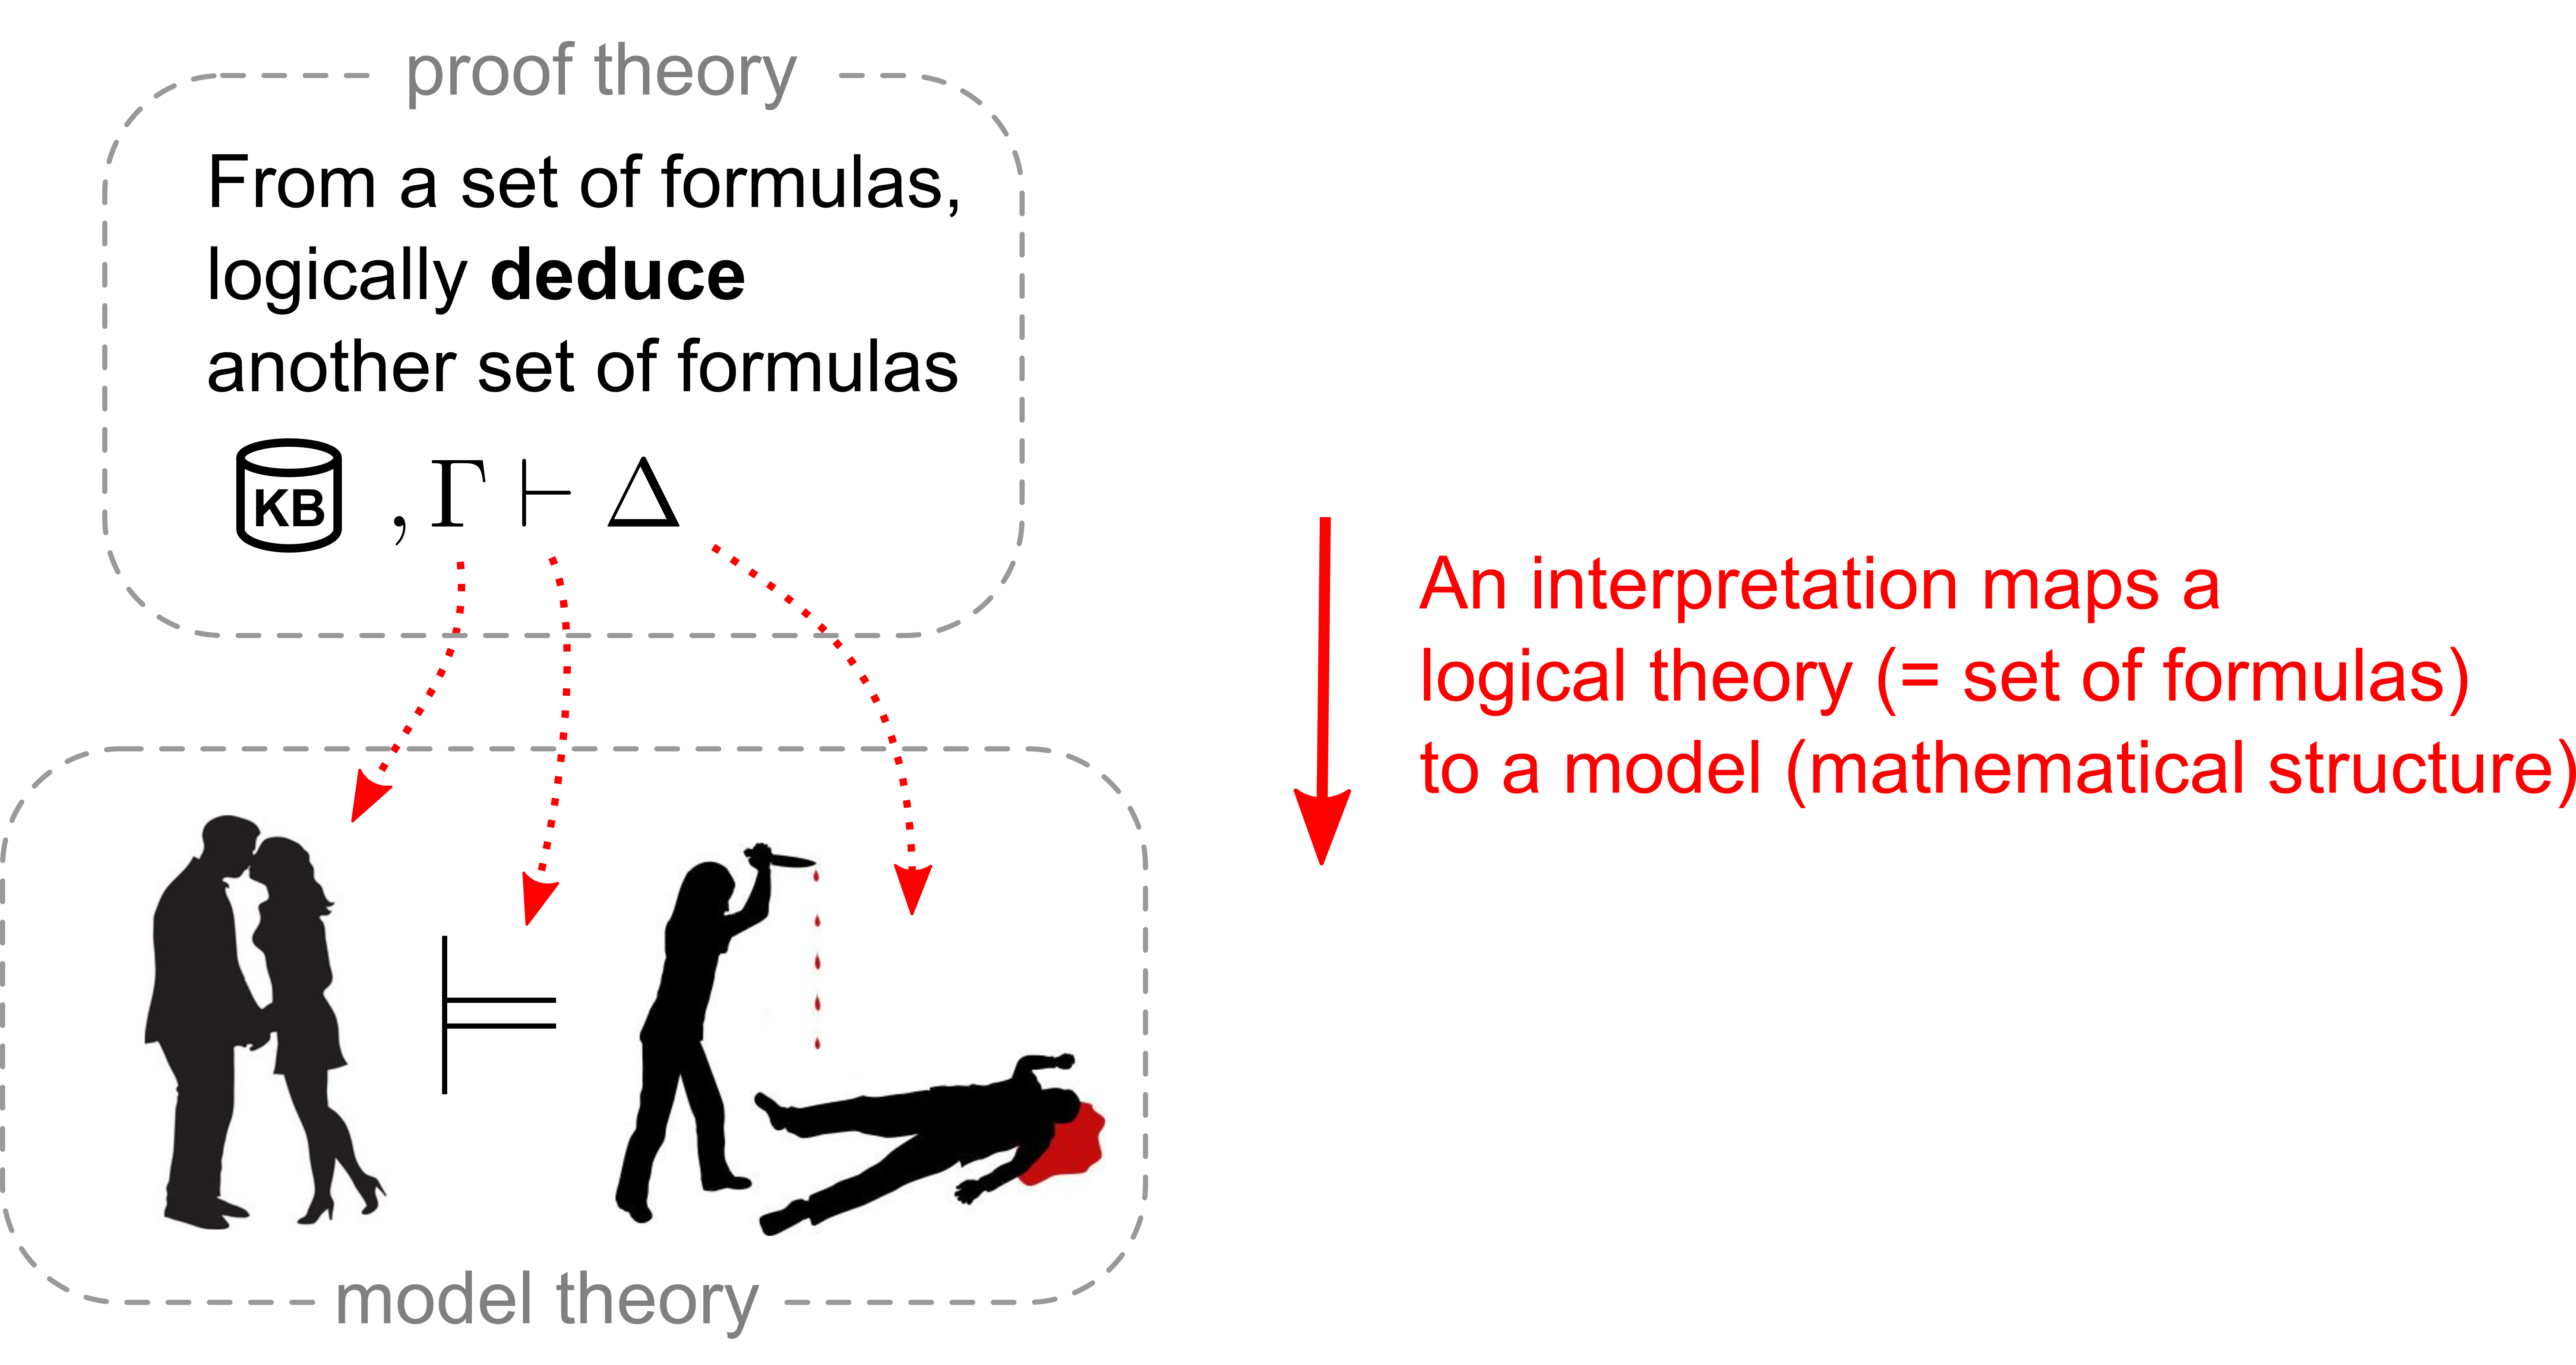
\includegraphics[scale=0.7]{model-theory.png}}}
\end{equation}
(逻辑是指丈夫有婚外情,推导出妻子因妒忌谋杀丈夫)

我理解 model 的意思,大概像「脑海中的小电影」。 例如,当我提及「妻子在家斩杀丈夫」这句子时,读者在脑中 re-construct 这个场景。 这时如果有 query 问: 「妻子当时是不是在酒吧喝酒? 」 或者 「现场是不是会遗下大量血迹?」  人脑 'ul{可以从 models 中直接 read off 这些答案}。 

广义上来说,model 就是一个和 ``the real thing'' 有某种程度相似的结构,例如尺码缩小了或变形了。  而 logic theory 是一堆命题,它表面上不像 real thing,但从广义来说,它也可以叫 model。

\subsection{\cc{模型是怎样产生的?}{Where do models come from?}}

在认知科学里,「模型」这概念并没有数学上严谨的定义,所以我提出一个观点: \unline{所有模型都是由 pattern recognition 的 }\textbf{\unline{ 逆运算}}\unline{ 产生的}:
\begin{equation}
\begin{tikzcd}
\boxed{raw data} \; \arrow[shift left]{rr}{\text{inductive learning}} && \; \boxed{theory} \arrow[shift left]{ll}{\text{model instantiation}}
\end{tikzcd}
\end{equation}
Pattern recognition 也可以叫 inductive learning。  Models 存在於 raw data 的空间中,这是合理的,因为 models 其实就是一些「被反向想像出来的 data」。  各种机器学习的算法,产生结构和性质不同的 theories,而这些 theories 逆向产生的 models 也会有不同的性质:
\begin{eqnarray}
\begin{tikzcd}
\boxed{raw data} \; D \arrow[shift left]{rr}{\ell_L} && T_L \; \boxed{logic theory} \arrow[shift left]{ll}{\ell^{-1}_L}
\end{tikzcd}
\\
\begin{tikzcd}
\boxed{raw data} \; D \arrow[shift left]{rr}{\ell_{NN}} && T_{NN} \; \boxed{NN theory} \arrow[shift left]{ll}{\ell^{-1}_{NN}}
\end{tikzcd}
%\boxed{raw data} \; D \stackrel{\ell_{L}}{\longrightarrow} T_{L} \; \boxed{logic theory} \\
%\boxed{raw data} \; D \stackrel{\ell_{NN}}{\longrightarrow} T_{NN} \; \boxed{NN theory}
%D \stackrel{\ell}{\longrightarrow} T
\end{eqnarray}
可以想像 logic theories 和 neural theories 之间有某种 \textbf{近似的等效} $\approx$: 
\begin{eqnarray}
& \begin{tikzcd}
	\text{logic theory} \arrow[leftrightarrow]{rr}{\text{approx. isomorphism}} && \text{NN theory} \\
	& \text{raw data} \arrow{ul}{\text{logic learning}} \arrow{ur}[swap]{\text{NN learning}}
\end{tikzcd} &
\nonumber \\
& \begin{tikzcd}
	T_{\text{L}} \arrow[leftrightarrow]{rr}{\approx} && T_{NN} \\
		& D \arrow{ul}{\ell_{L}} \arrow{ur}[swap]{\ell_{NN}}
\end{tikzcd} 
\end{eqnarray}
我们的目的是找出这个 $\approx$ 可资利用的优势。

早在 2000 年,Jocelyn \parencite{Ireson-Paine2000} 已提出了 在机器学习中 generalization 可以理解成 adjunction,这看法和我的理论是一致的。

\subsection{与神经网络的关系} \label{Logic and NN}

主导思想: \unline{用 神经网络 $\,F$ 模拟 逻辑的 $\,\vdash$}。

深度神经网络 可以自动学习出 \textbf{知识表述} (representations),这 representation 的 \textbf{涌现} (emergence) 是由 \textbf{目标函数} 的最优化「迫」出来的。

一个重要的问题是:  \unline{逻辑的 代数结构 如何 影响 $\,F$ 的结构,及 $\,F$ 的 learning algorithm}?

$\vdash $ 似乎是一个 multi-valued function,但 $F$ 会是 single-valued。  在这个 \textbf{选择} 过程中,似乎蕴含了 \textbf{proof search}(更正确地说是 consequence search,实际 implement 时可以用 best-first search, A*-search 等)。

\unline{逻辑的代数结构 似乎就是 lattice 结构}(如果不考虑 predicate logic 的 fibration),所以 consequence search 是在一个 lattice 中进行。  

其实共有 3 个层次:
\begin{itemize}
	\item \textbf{Propositional lattice}: 这是 deduction 的 search space。
	\item $\KB$ \textbf{lattice}: 每个 (propositional) lattice 是由 $x \rightarrow y$ 这样的逻辑 rules 决定,换句话说是 $\KB$ 的内容。  换句话说,每个 $\KB$ 决定一个 lattice。  但,不同的 $\KB$ 也组成另一个 更大的 lattice。  这就是 inductive learning 里面的 \textbf{hypothesis space}。
	\item 而,不同的 logics 也可以组成一个「更大更大」的 lattice (in the sense of universal algebra),但我觉得这不是重点,因为在 logic 的方向上很容易就已经达到 Turing universal 的程度,所以我们暂时不必深究用哪个 logic。  这是 meta-logical learning 的 search space。
\end{itemize}

$F$ 的迴路构成一个 RNN (recurrent neural network)。  RNN 的特性是它会自动地 iteratively settle down to a certain interpretation, which seems to be an advantage.  每次 iteration 是在寻找 global minimum,换句话说,iteration 期间 是 尝试 一些 combinations of possible solutions, analogous to \textbf{proof search} in LBAI.

总结一下以上的论述:
\begin{itemize}
	\item Logic's algebraic structure gives rise to lattice structure, which is the structure of the search space of deduction.
	\item The set of all $\KB$'s form a lattice which is the hypothesis space of inductive learning.  This lattice structure is induced by the lattice structure of logic.  The search for optimal $F$ occurs in this lattice.  	
\end{itemize}

%用下面这样的图形代表「模型」:
%\begin{equation}
%\vcenter{\hbox{\includegraphics[scale=0.75]{../courtship.jpg}}}  \quad 
%\vcenter{\hbox{\includegraphics[scale=0.75]{../murder.jpg}}} 
%\end{equation}

%但我们并不太熟悉这些由 神经网络 涌现的 representations 内部是什么结构,我假设这种 representation 和 模型论 描述的结构 是 \textbf{同构} (isomorphic) 的; 当然,这个说法有点 vacuous。
%\begin{equation}
%\vcenter{\hbox{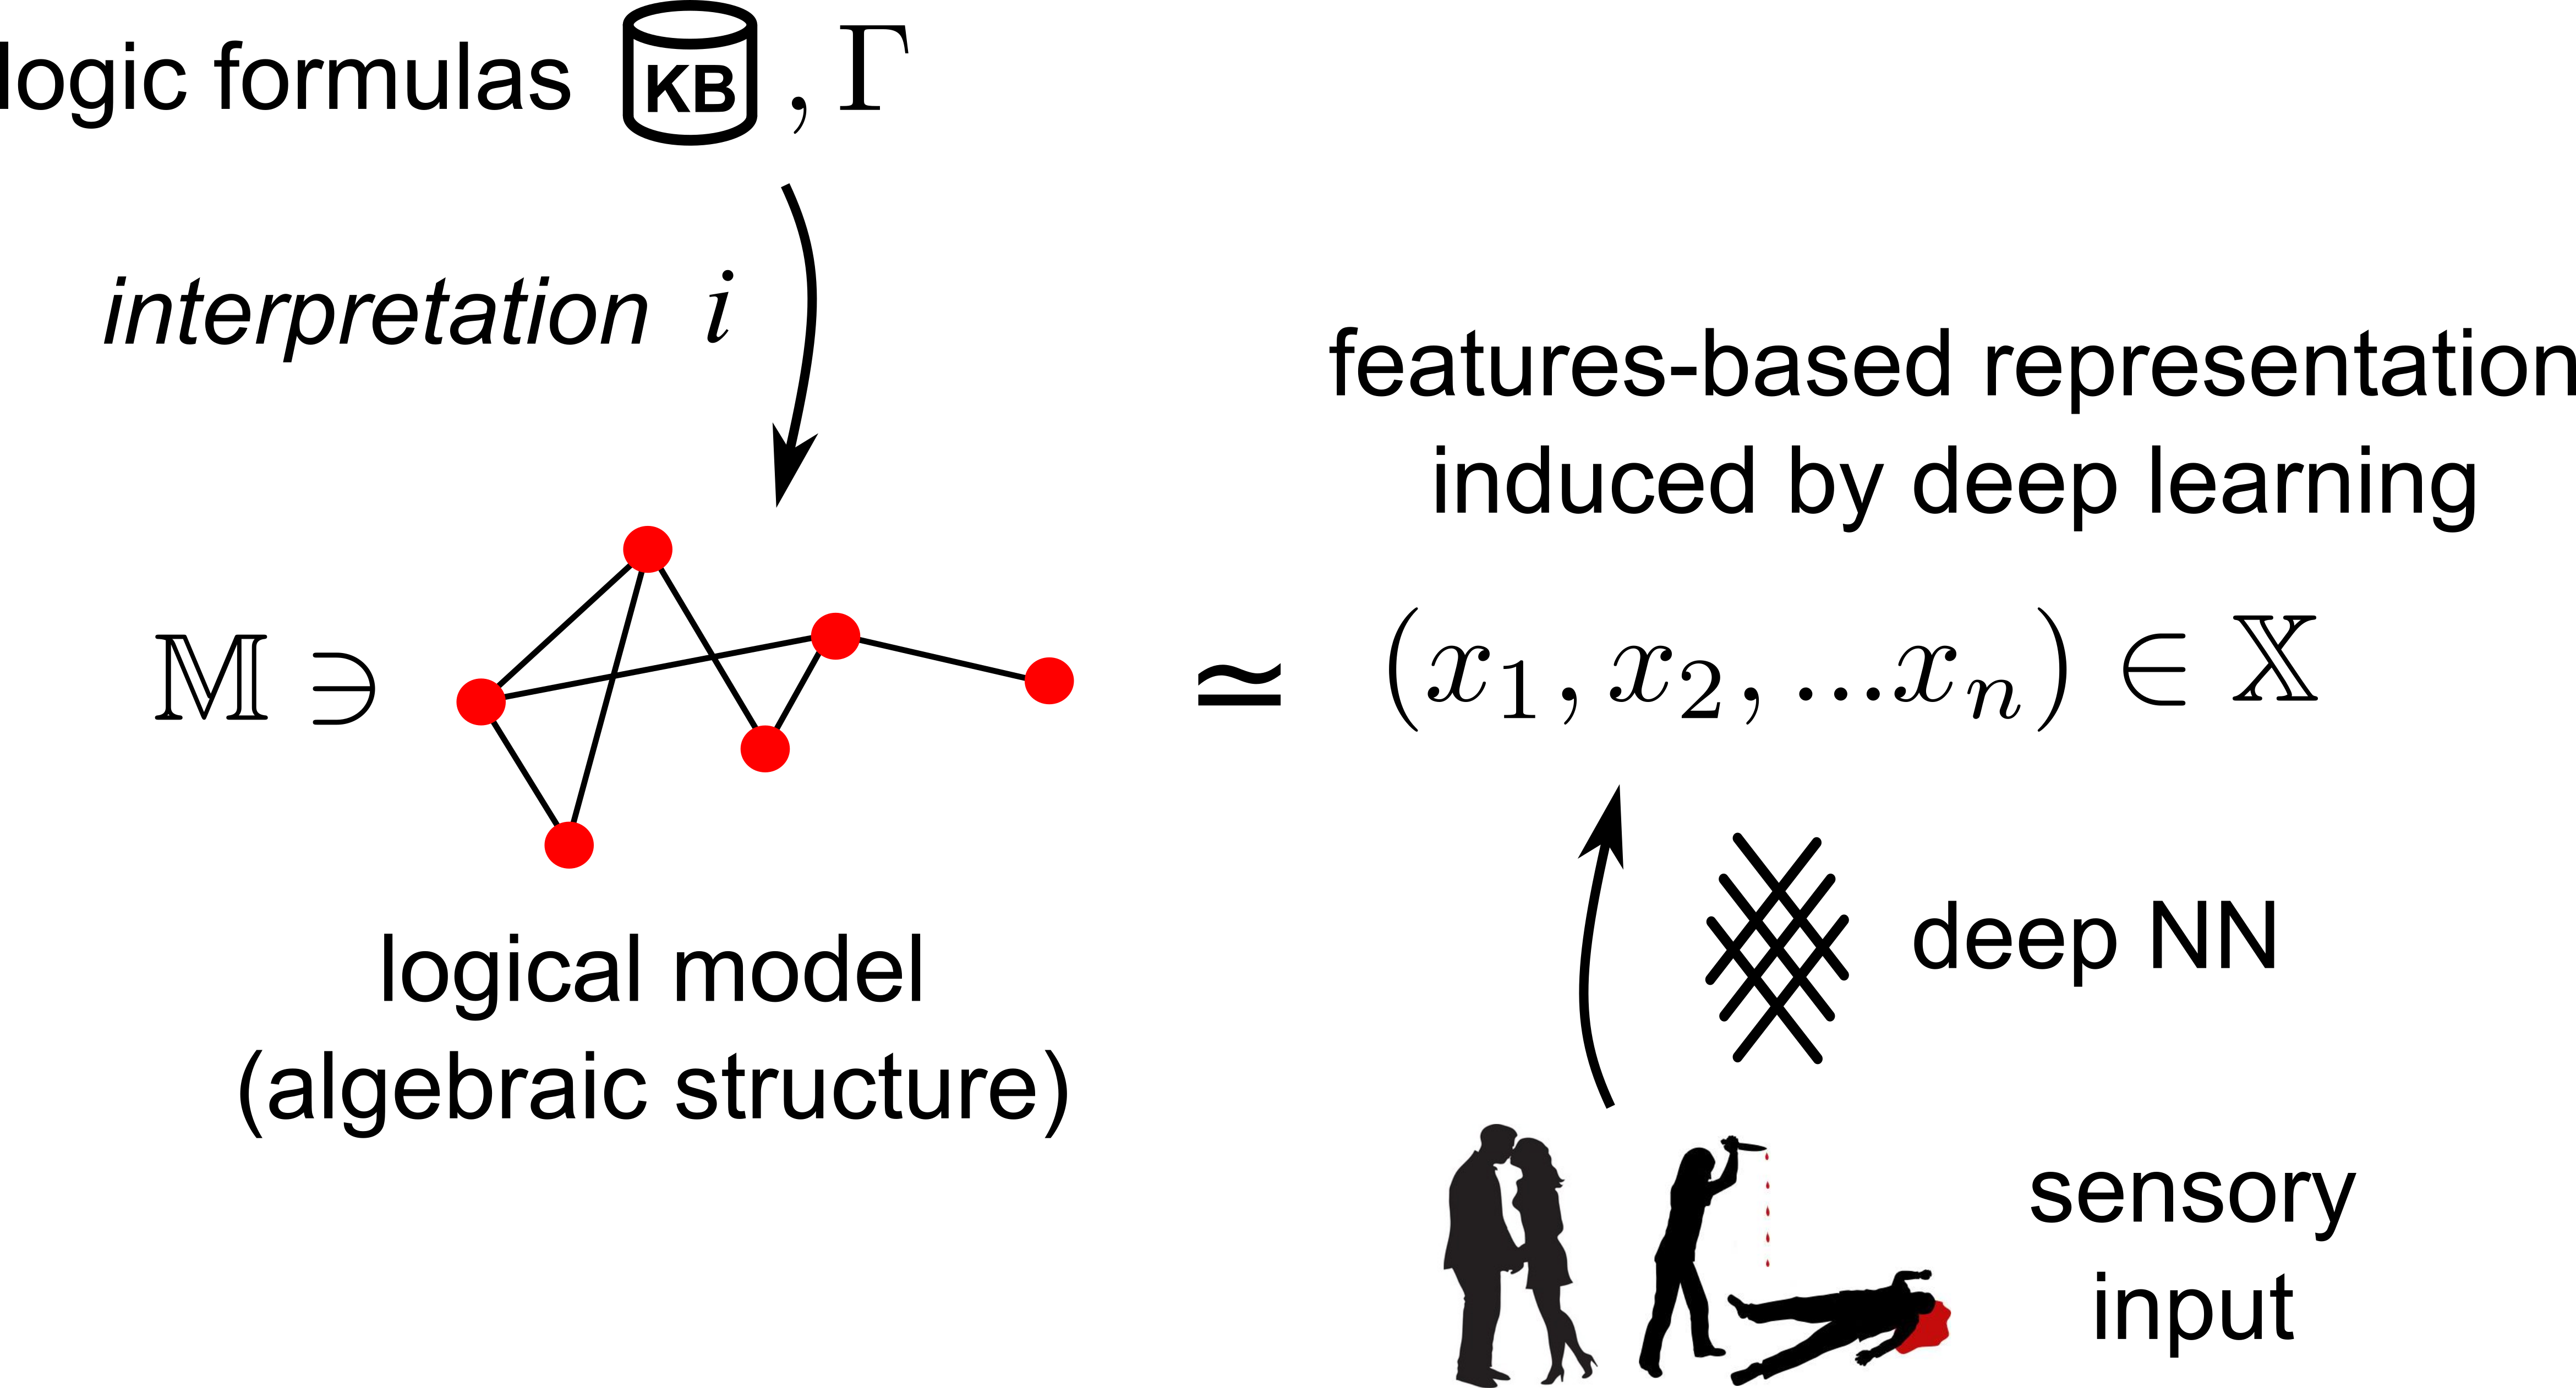
\includegraphics[scale=0.7]{model-theory-2.png}}}
%\end{equation}

		\subsection{functorial semantics, ``internal language''}

将 模型论 用 范畴论 的方法表述,得到 \textbf{functorial semantics}。 

在 \parencite{Crole1993} 一书里有解释:

\textbf{Internal language} 是指 一个范畴 $\mathbf{C}$ 诱导出的 algebraic theory $Th(\mathbf{C})$,叫作 $\mathbf{C}$ 的 internal language.  This language is extremely useful because it allows us to reason about the category $\mathbf{C}$ as though it were the category $\mathbf{Set}$ of sets and functions.  For example, if $f: A \rightarrow B$ is a morphism of $\mathbf{C}$, then there is a \textbf{proved term} $x: A \vdash f(x): B$ in $Th(\mathbf{C})$.

\underconst (还要解释一下,这 internal language 似乎是 Curry-Howard isomorphism 的一种形式....)

	\section{Architecture of logic-based AI (LBAI) systems}

经典 LBAI 的基本运作是这样的(即 经由 $\KB$ 的逻辑法则,从 current state 推导到下一个结论):
\begin{equation}
\vcenter{\hbox{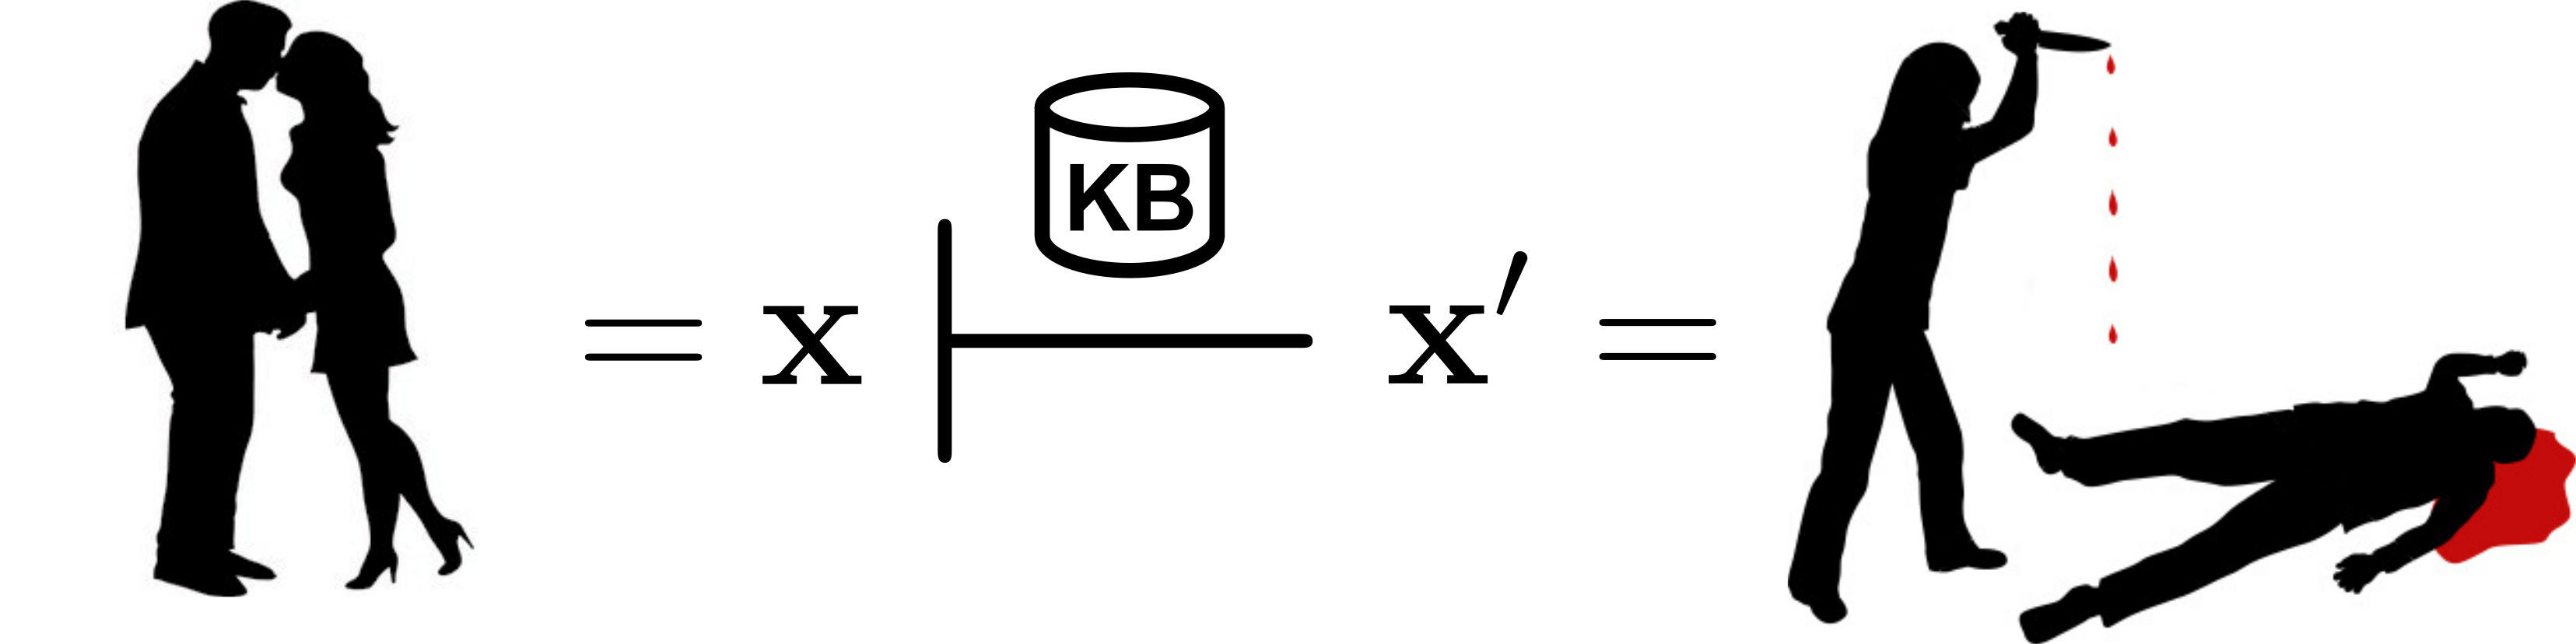
\includegraphics[scale=0.7]{LBAI-basic-operation.png}}}
\end{equation}
$\KB$ 是一些 \textbf{条件命题} (logic rules) 的集合。

\textbf{逻辑推导} 分解成几个动作 完成:
\begin{itemize}
	\item unification: 即 pattern matching,寻找 KB 中 可用的 条件命题
	\item resolution: 应用条件命题 推导出新的结论
\end{itemize}
问题是,经典 LBAI 中的 $\vdash$ 是 ``symbolic'' 的。 换句话说: 经典 LBAI 最大的问题是,\uline{它处理的元素之间没有 semantic distance},而只有 syntactic distance,而后者基本上是没有用处的。  为了解决这问题,似乎需要使用 model theory,因为 models 的内部可以用 semantic distance 量度。 

在 \textbf{认知科学} 里,关於 pattern recognition 的问题,一直有 model-based view 和 theory-based view 等论点的争议。 究竟人的认知 是基於:
\begin{itemize}
	\item logic theory,即一些 \textbf{逻辑法则} 的集合
	\item prototypes / exemplars,记忆一堆例子,然后新的例子 用 similarity metric 量度
	\item models ?
\end{itemize}
例如 人 怎样辨认「水果」这概念?  例如「tomato」不是甜的,所以属於 borderline 水果,这似乎是根据 逻辑法则 决定的。 

在 经典 LBAI 里,如果要回答「妻子在案发当时是不是在酒吧喝酒?」 需要用到一些逻辑法则,例如:「如果 A 用刀斩 B,则 A 需要在 B 的近距离」,这样可以推导出「妻子不可能在酒吧」。  但问题是,我们假设 知识库 $\KB$ 中有这样的一些法则 似乎很牵强。  LBAI 支持者通常的回答是: 知识库中有成千上万的逻辑法则,多不胜数,这只是其中一条。  但细想之下这个做法似乎有点不切实际。

另方面,如果 我 凝视 面前自己的手掌,我脑中 建立的 model 是类似一个 立体的 block 加上几个 cylinders。  其实这个 model 也可以表述为一组 \textbf{逻辑命题},所以 model 和 logic theory 之间没有明确分野。  甚至一个神经网络 的 neuron,它只负责辨认一个微小的 feature,但这个 feature 也可以转变为 逻辑命题。 

	\section{\cc{代数逻辑、逻辑的几何化}{Algebraic logic, geometrization}}

谓词逻辑 的 \textbf{代数化} (algebraization) 有两个做法: Alfred Tarski 的 \textbf{cylindric algebra} 和 Paul Halmos 的 \textbf{polyadic algebra}。  如果不用 谓词逻辑,也可以有 \textbf{relation algebra} 这种代数。 

\subsection{Cylindric algebra}

Cylindric algebra 由 Tarski 发明,目的是给出 first-order logic 的一种 \textbf{代数形式} (algebraization)。 

例如,一个关系 $x_1 R\, x_2$,也可以记为 $R(x_1, x_2)$,它存在於 $X_1 \times X_2$ 这两个 domain 的 Cartesian 乘积之中:
\begin{equation}
\vcenter{\hbox{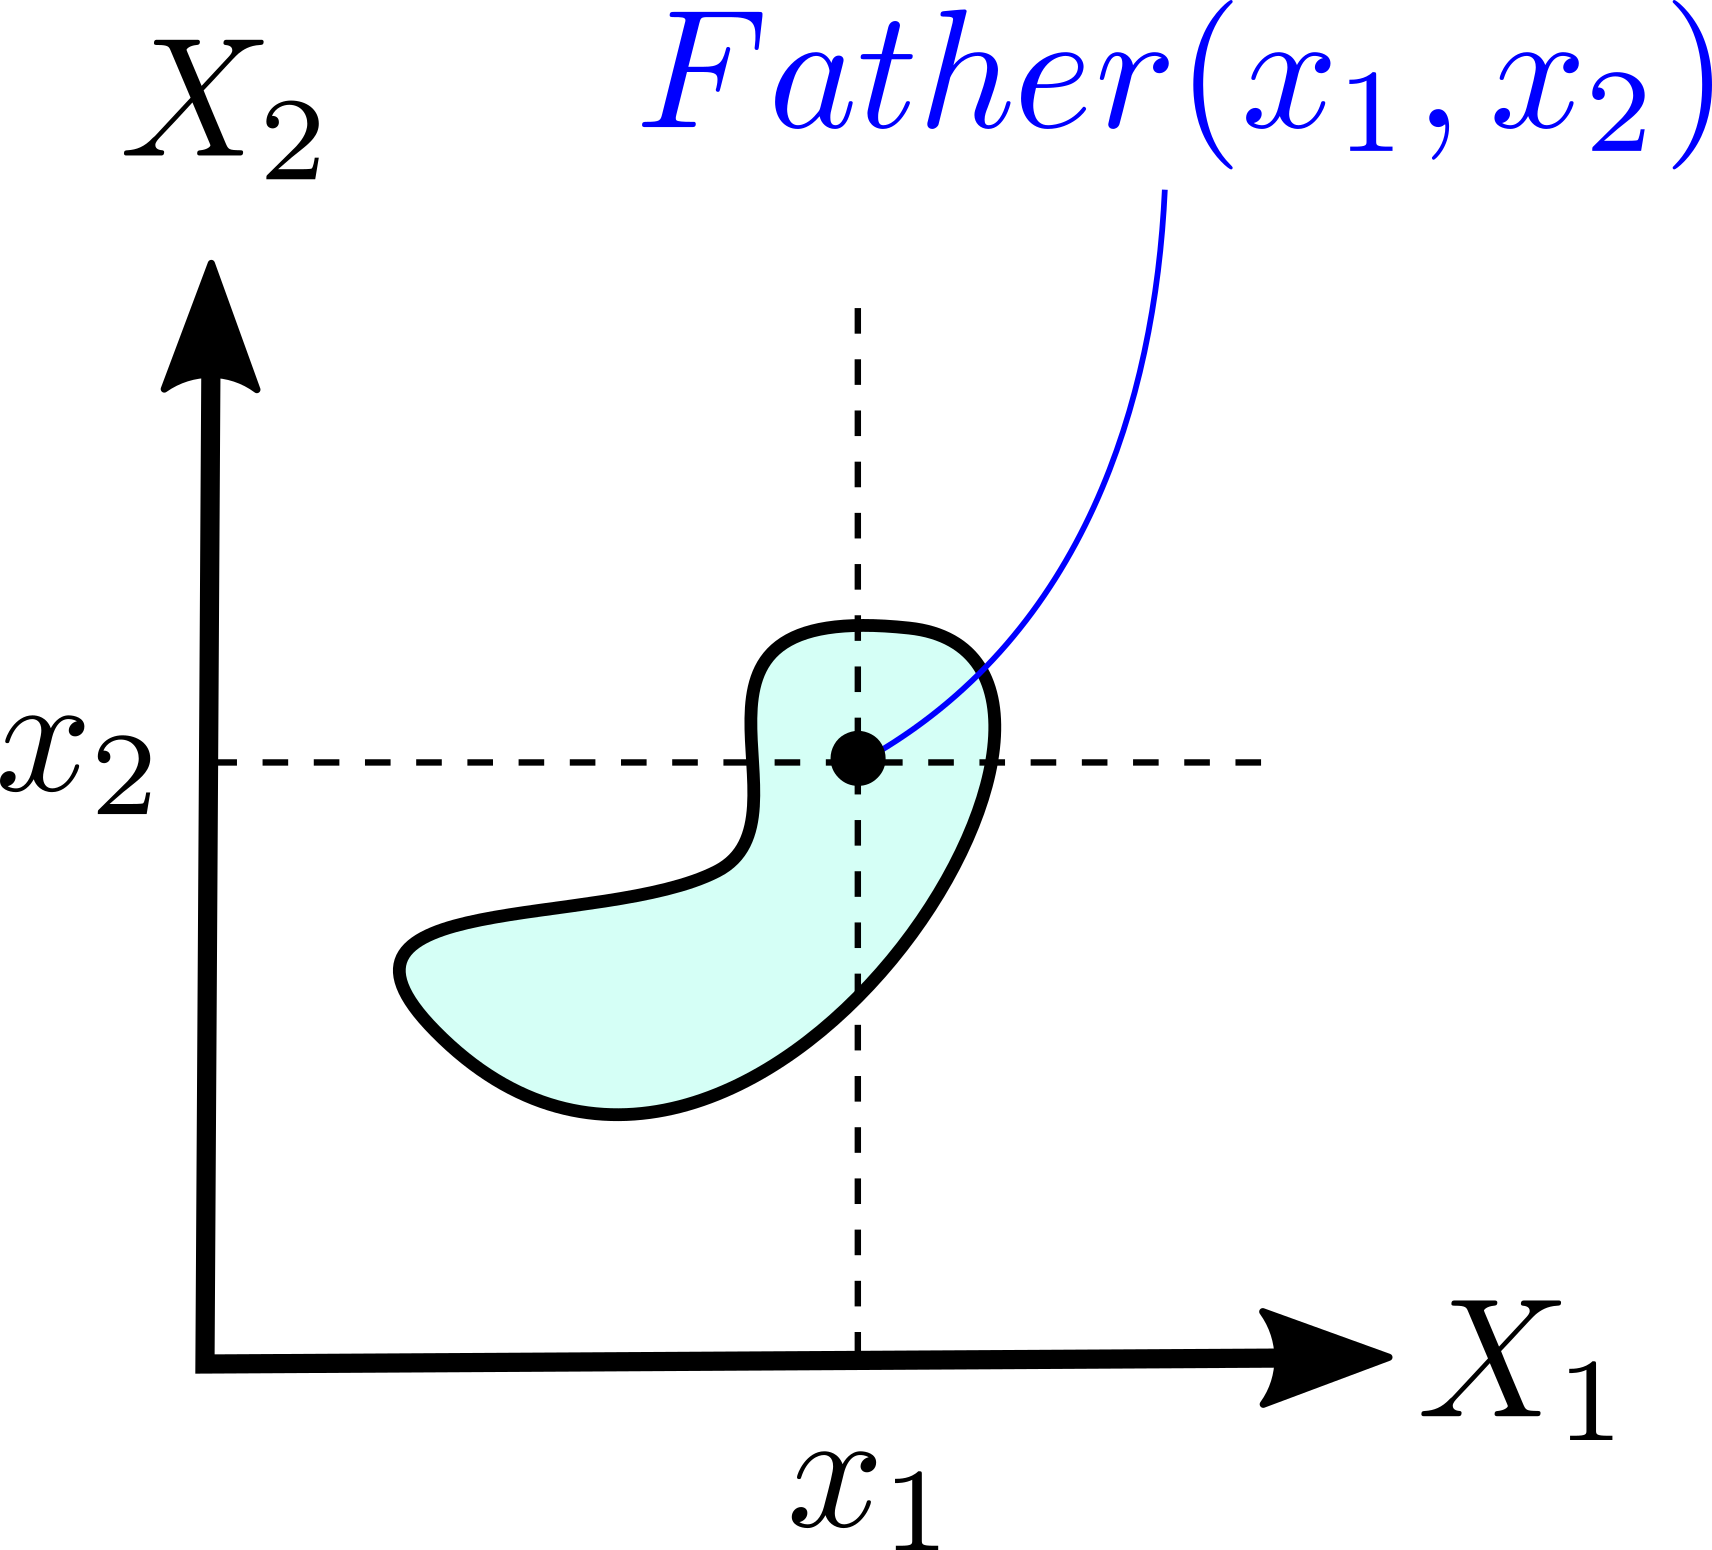
\includegraphics[scale=0.7]{cylindric-relation.png}}}
\end{equation}
Topologically, cylinders 的产生是来自 domains 的 Cartesian 乘积,\\
例如 $Father(x_1, x_2)$ 是 $X_1 \times X_2$ 内的一个区域 $D$,但 $x_3$ 是 ``don't care'',所以「乘以」domain $X_3$ 的 \textbf{全体},亦即 $D \times X_3$,因而产生 cylinder:
\begin{equation}
\vcenter{\hbox{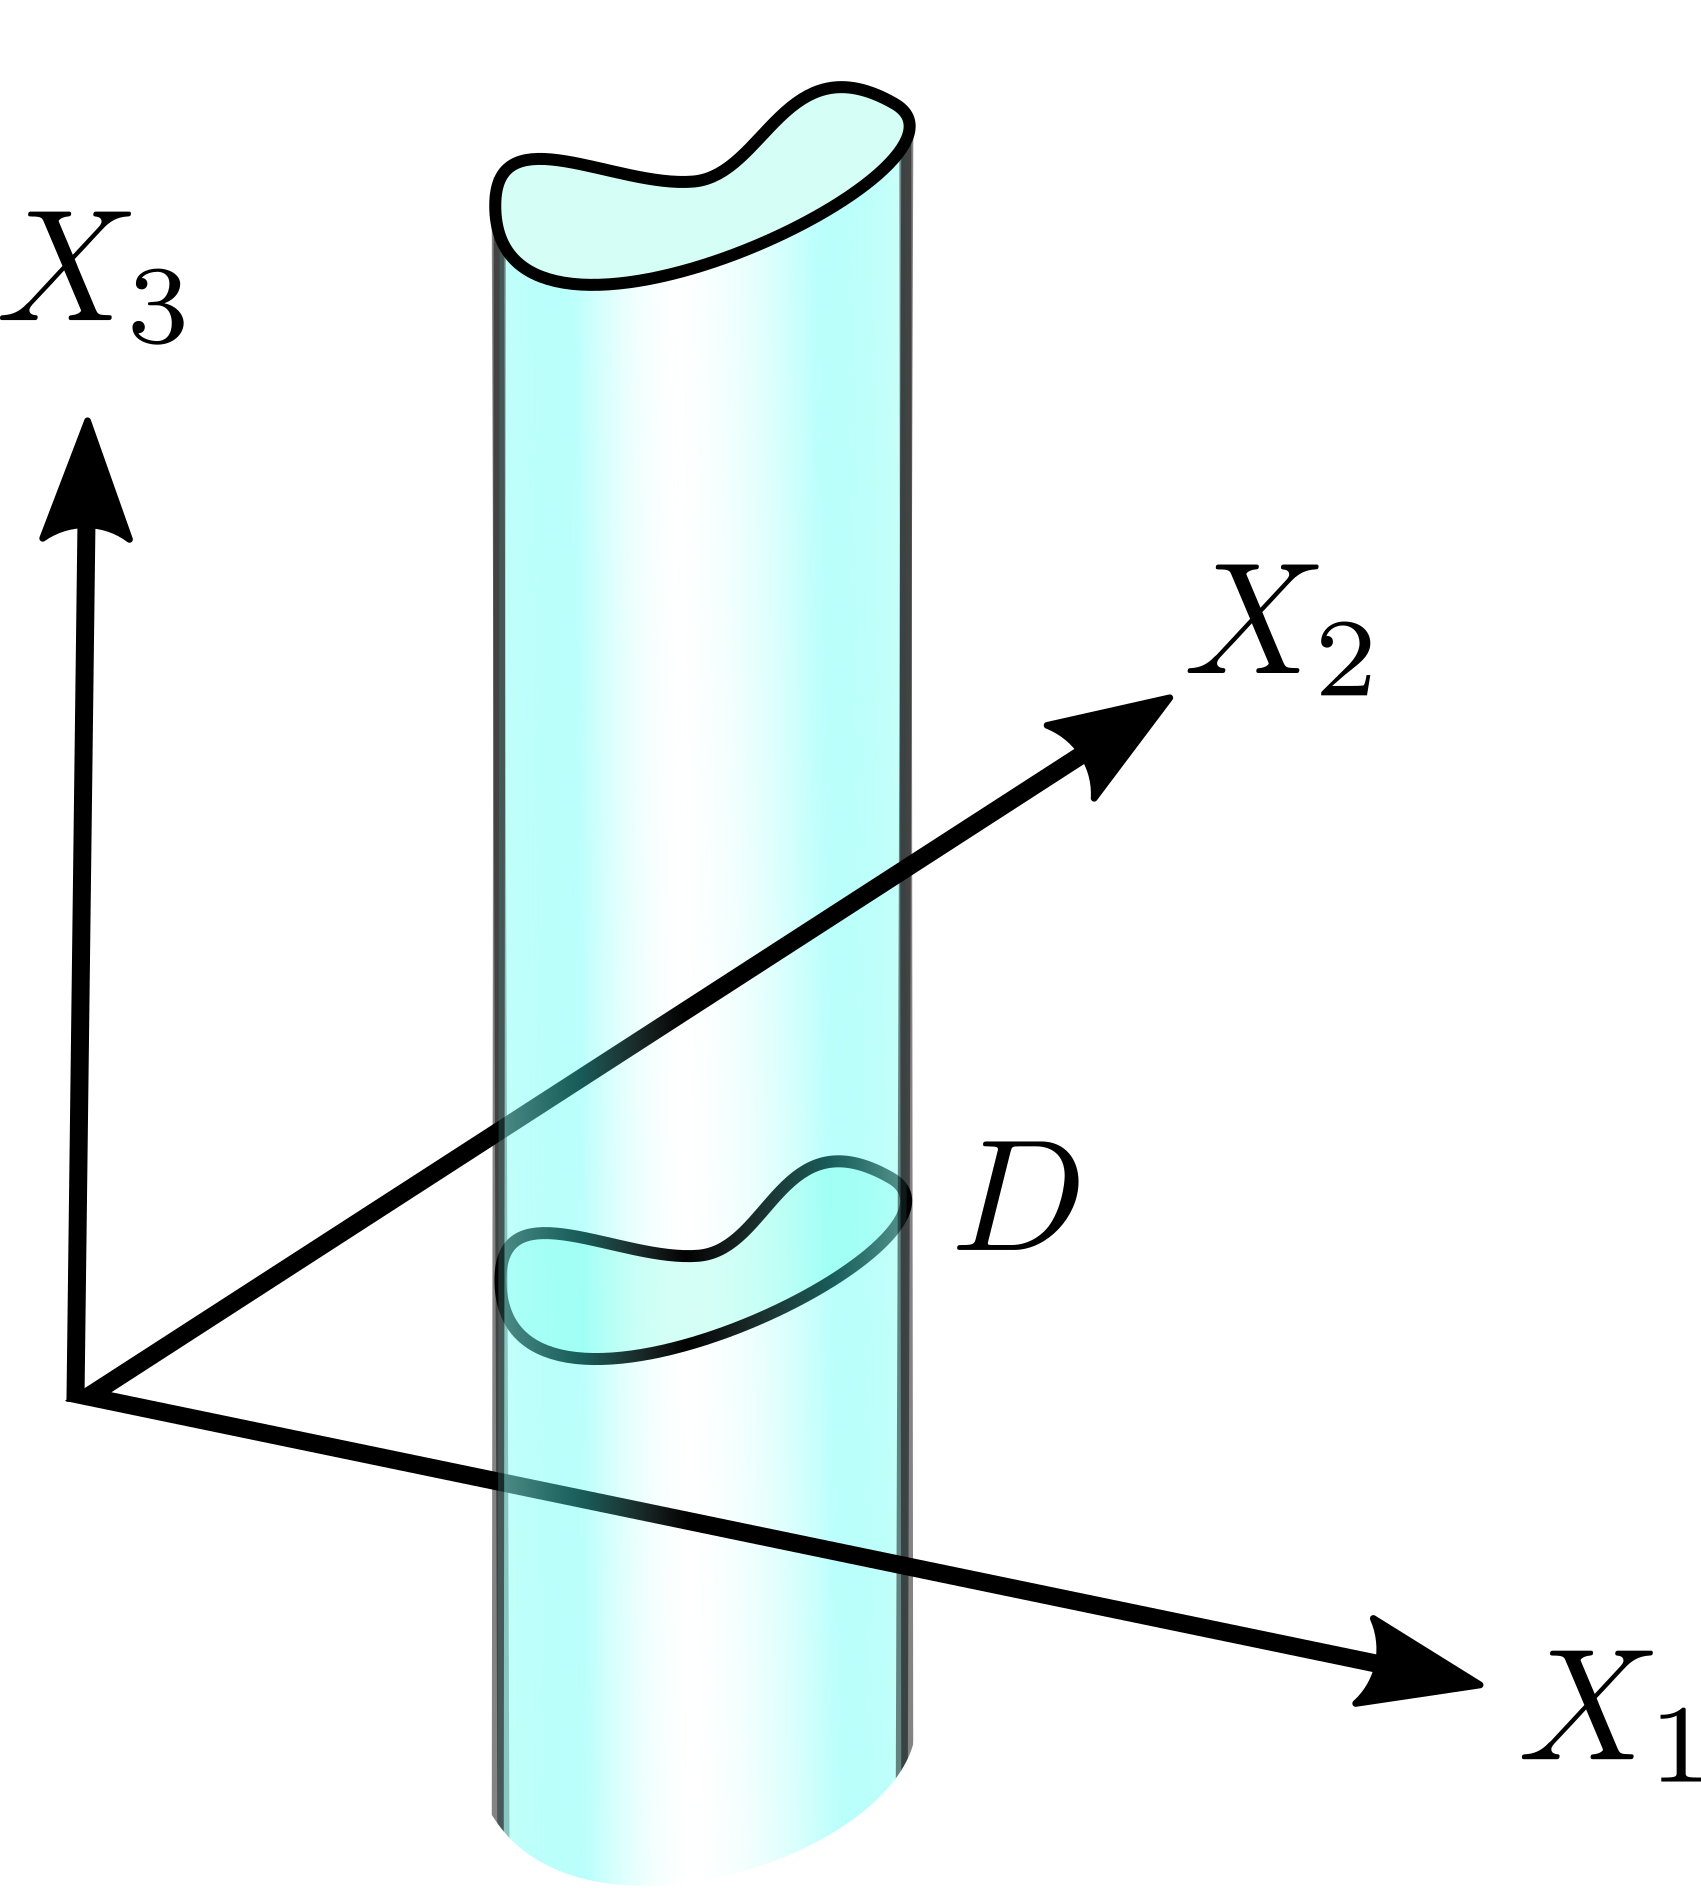
\includegraphics[scale=0.7]{cylindrification-example.png}}}
\end{equation}

两个关系的 composition $R_1 \circ R_2$ 是他们的 cylinders 的 intersection:
\begin{equation}
\vcenter{\hbox{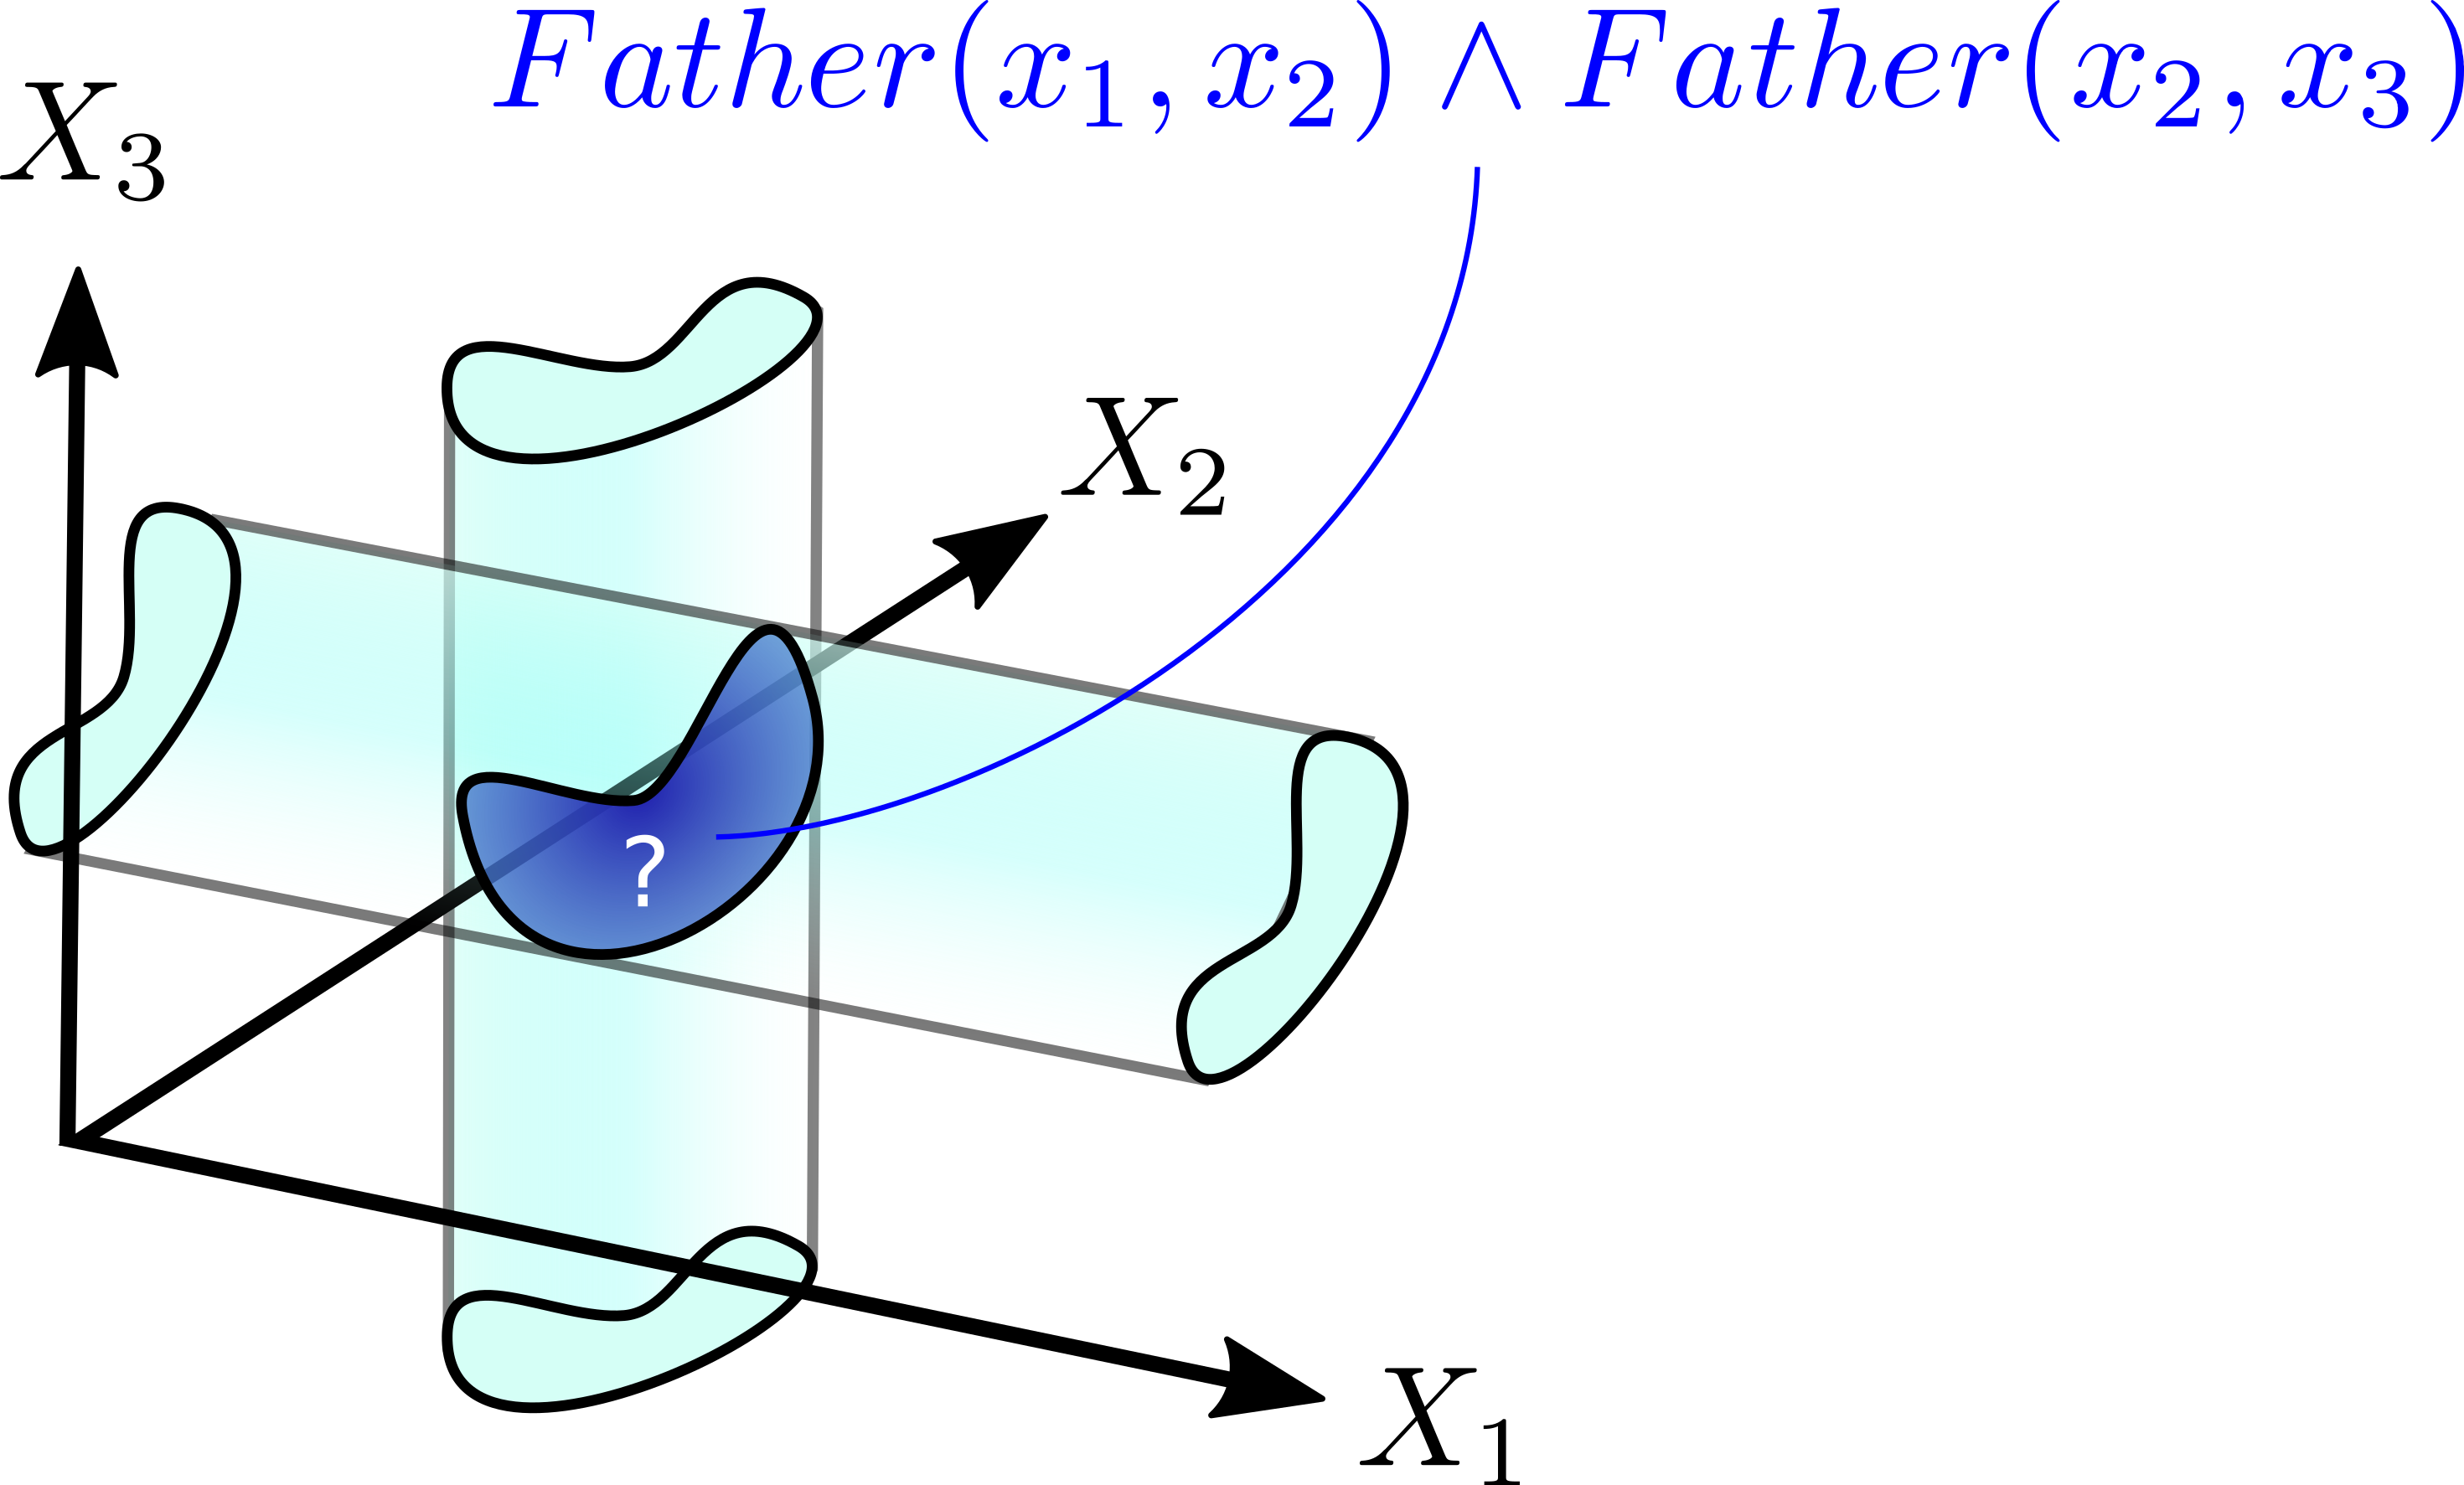
\includegraphics[scale=0.7]{cylindric-relation-intersection.png}}}
\end{equation}
这个 intersection 的形状可以很复杂,例如当两个 L 形的 cylinders intersect 时,会产生这个体积:
\begin{equation}
\vcenter{\hbox{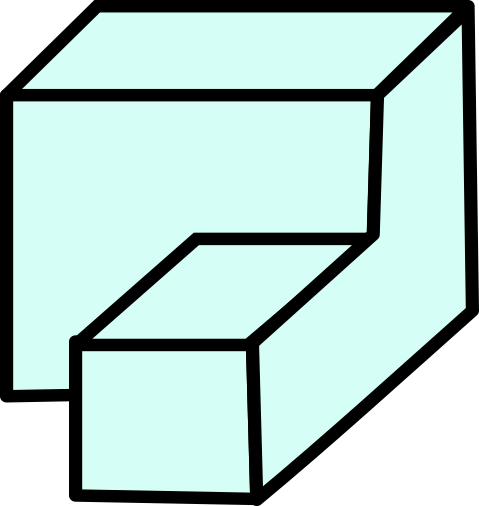
\includegraphics[scale=0.7]{cylindric-relation-intersection-example.png}}}
\end{equation}

量词 $\forall$ 的 cylindrification 如下图所示:
\begin{equation}
\vcenter{\hbox{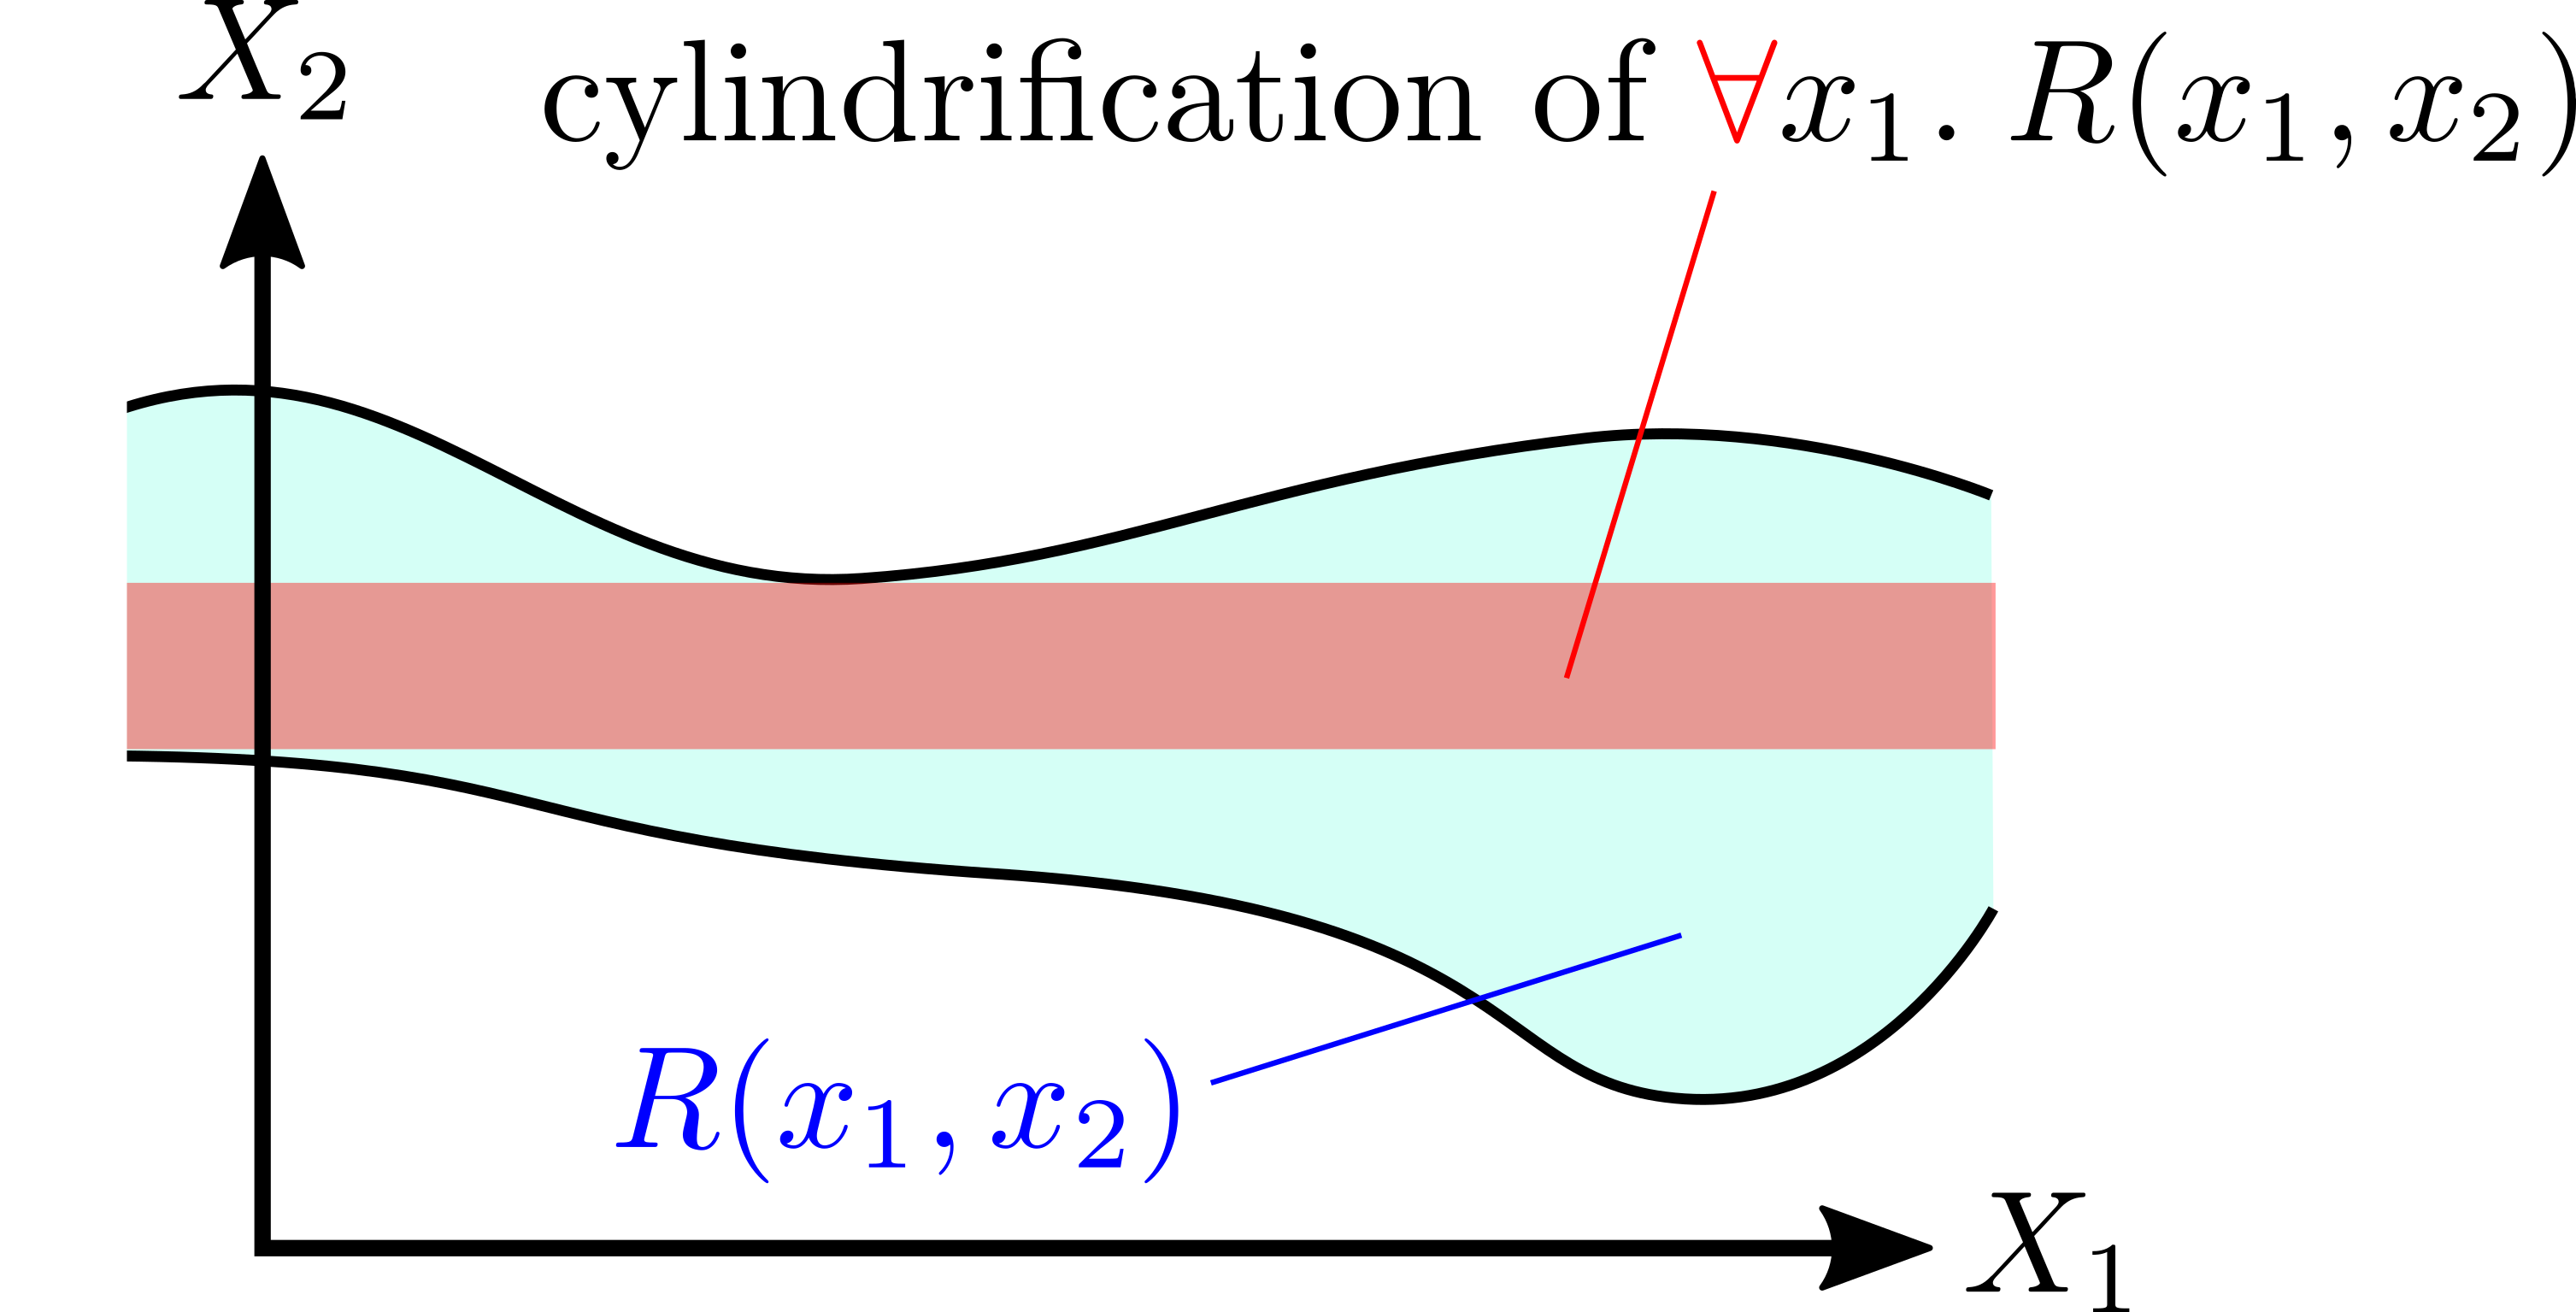
\includegraphics[scale=0.65]{cylindrification-forall.png}}}
\end{equation}
在上例中,$\forall$ 的 cylindrification 是这个集合:
\begin{equation}
{\color[rgb]{0.9,0.7,0.7} 
	
\begin{tikzpicture}[overlay]
	\draw[fill] (-0.53,-0.1) rectangle (-0.05,0.33);
	\end{tikzpicture}
} {}_{\forall} = \{ (x_1, x_2) |\; \forall \hat{x_1}.\;  R(\hat{x_1}, x_2)  \} 
\end{equation}
同样地,
\begin{equation}
\vcenter{\hbox{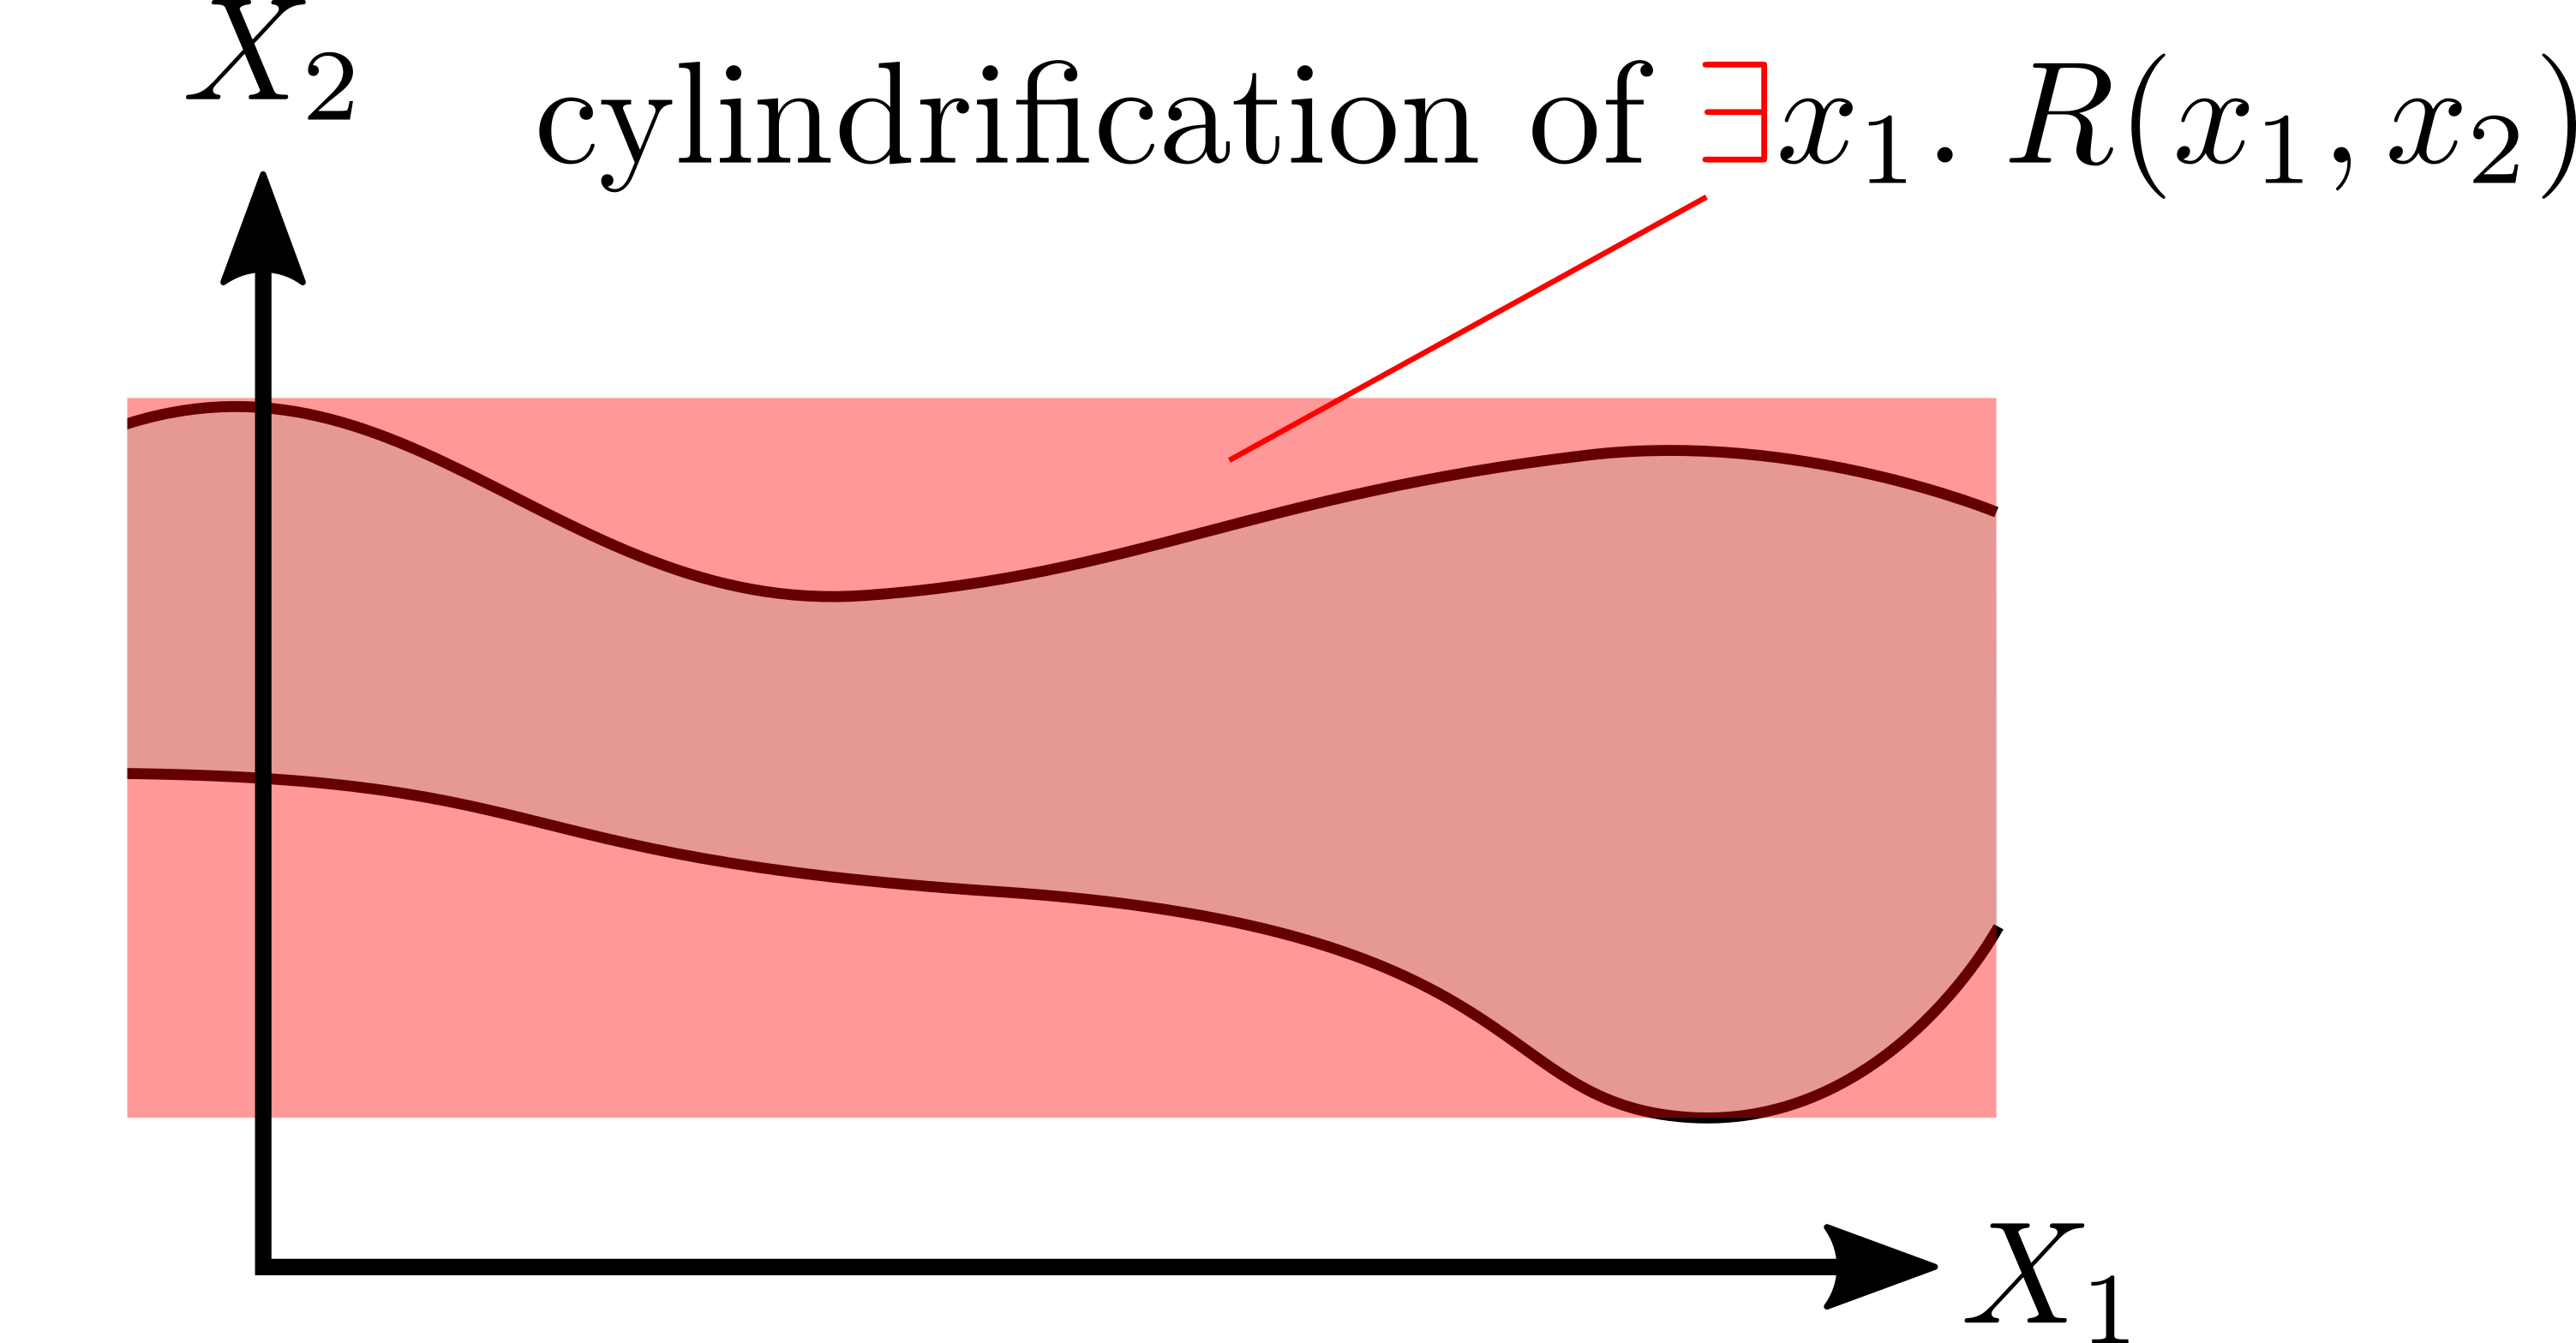
\includegraphics[scale=0.65]{cylindrification-exists.png}}}
\end{equation}
$\exists$ 的 cylindrification 是这个集合:
\begin{equation}
{\color[rgb]{0.9,0.7,0.7} 
	
\begin{tikzpicture}[overlay]
	\draw[fill] (-0.53,-0.1) rectangle (-0.05,0.33);
	\end{tikzpicture}
} {}_{\exists} = \{ (x_1, x_2) |\; \exists \hat{x_1}.\;  R(\hat{x_1}, x_2)  \} 
\end{equation}

或者 \textbf{等效地},可以将 $\forall$ 和 $\exists$ 表示成 定义域内 $X_2$ 成分的 \textbf{投影}:
\begin{equation}
\vcenter{\hbox{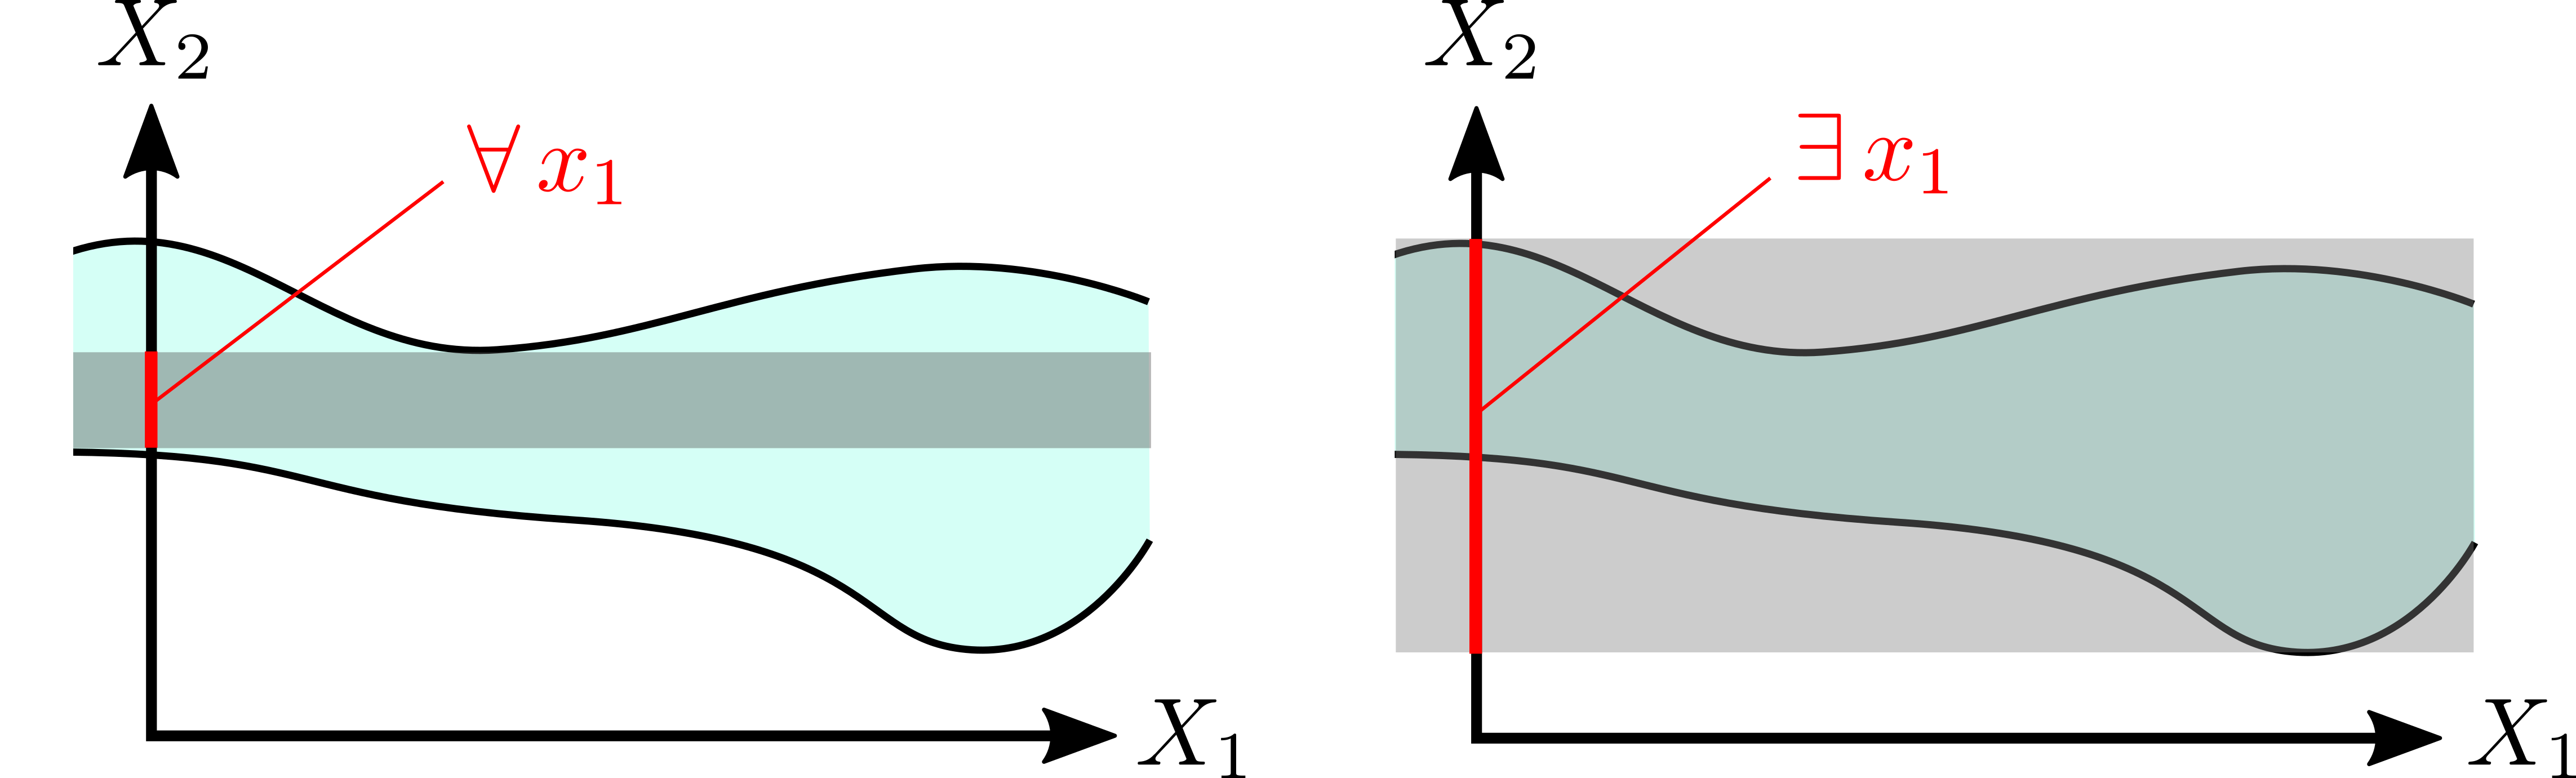
\includegraphics[scale=0.7]{cylindrification-projected.png}}}
\end{equation}

这时,我们定义 \textbf{投影} 函数: 
\begin{equation}
\pi_1 (x_1, x_2) = x_1,  \quad \quad \pi_2 (x_1, x_2) = x_2
\end{equation}

则上面的两个 投影后的集合 可以表示成:
\begin{eqnarray}

\begin{tikzpicture}[overlay]
\draw[red,line width=3pt] (-0.1,-0.1) -- (-0.1,0.4);
\end{tikzpicture}
{}_{\exists} &= {\exists}_{x_1} &= \{ x_2 |\; \exists \vec{x}.\;  \left[ x_2 = \pi_2(\vec{x}) \;\wedge\; \vec{x} \in R \right] \} \nonumber \\

\begin{tikzpicture}[overlay]
\draw[red,line width=3pt] (-0.11,-0.1) -- (-0.11,0.4);
\end{tikzpicture}
{}_{\forall} &= {\forall}_{x_1} &= \{ x_2 |\; \forall \vec{x}.\;  \left[ x_2 = \pi_2(\vec{x}) \;\rightarrow\; \vec{x} \in R \right] \} 
\end{eqnarray}
\begin{tabbing}
\hspace*{2cm}\=  \kill
注意: \> 在第二式中的 $\rightarrow$ 是必需的,不能用 $\wedge$ 代替,这是很微妙的区别,而两式并不完全对称。 \\
      \> 被量词 $\exists x$ 和 $\forall x$ \textbf{束缚} (bound) 的变量,\uline{是那个被 投映 忽略了的变量},而不是被投映到的变量。 \\
\end{tabbing}

上面两式可以用更简洁的方法描述:
\begin{eqnarray}
{\exists}_{x_1} &=& \pi_2(R) \nonumber \\
{\forall}_{x_1} &=& \pi_2(R')' 
\end{eqnarray}
\begin{tabbing}
\hspace*{3cm}\=  \kill
换句话说: \> $\exists$ 是 $R$ 经过投映 $\pi_2$ 的 \textbf{象} (image),\\
         \> $\forall$ 是 $R$ 的 \textbf{补集} (complement) 的投映的补集(如下图): \\
\end{tabbing}
\begin{equation}
\vcenter{\hbox{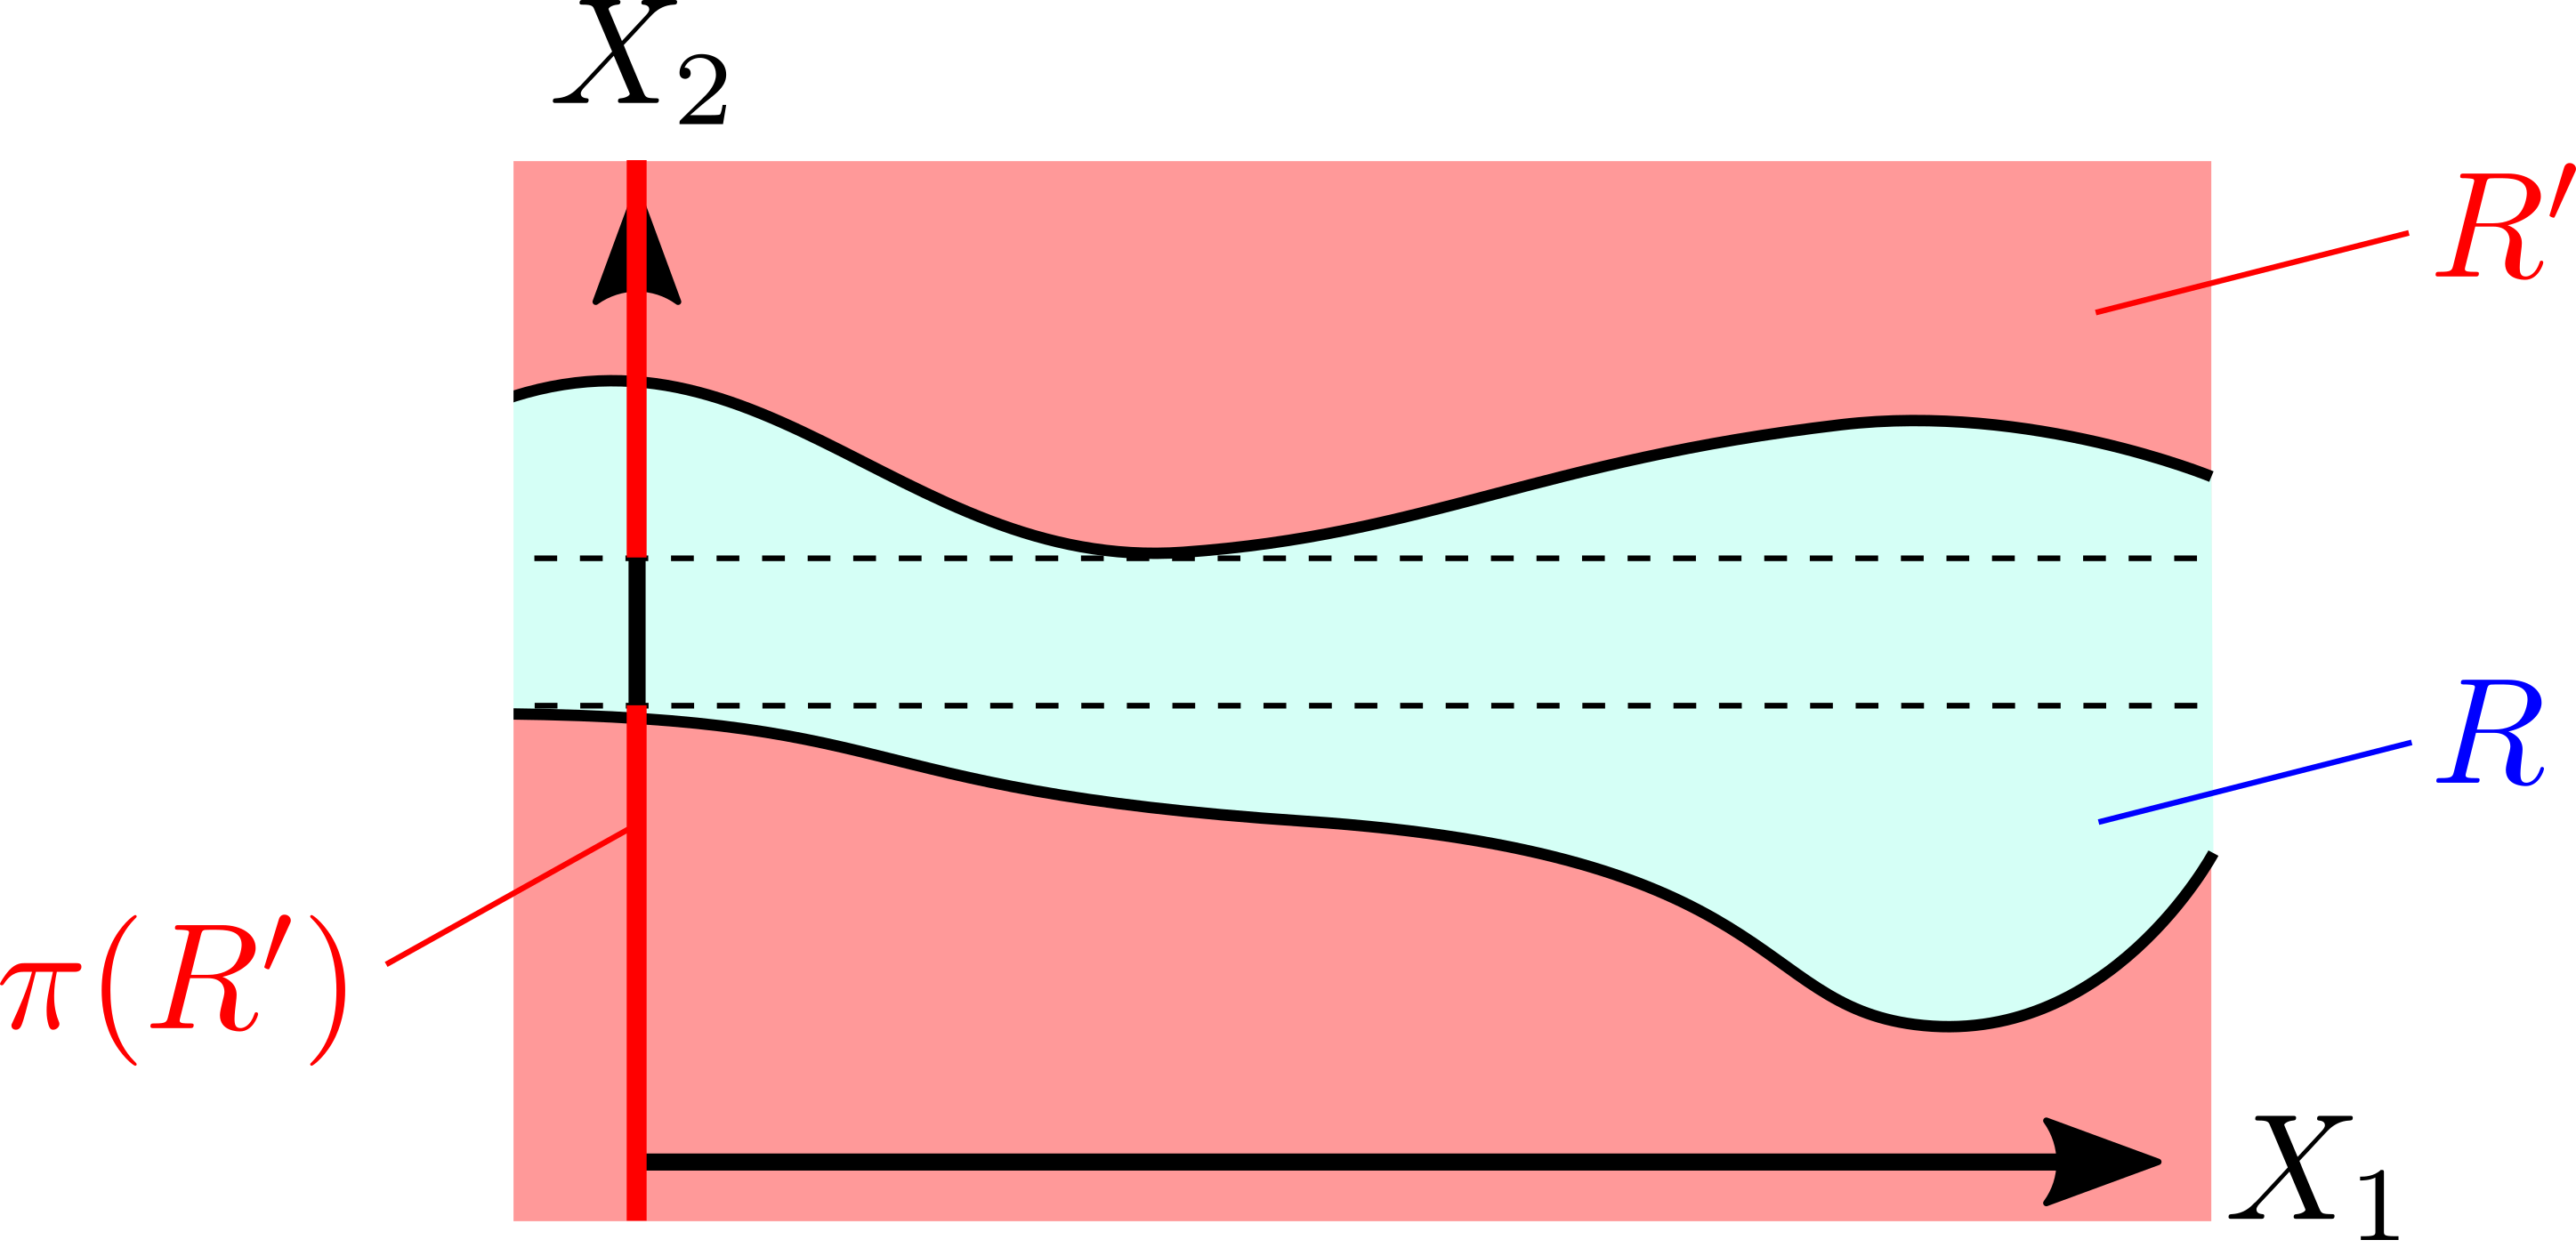
\includegraphics[scale=0.7]{cylindrification-forall-complement.png}}}
\end{equation}

F William Lawvere 在 1960's 年代提出了基於 范畴论 的更深入的想法,见 \S\ref{sec:categorical-logic}。

\subsection{Cylindrical algebraic decomposition (CAD)}

CAD 是在 real algebraic geometry 中很重要的一个 algorithm,或许和 cylindric algebra 有些关系。

\underconst

\subsection{Quantifier elimination}



	\section{\cc{范畴论、范畴逻辑}{Category theory, categorical logic}}
	\label{sec:categorical-logic}	

范畴逻辑的要点可概括为:
\begin{itemize}
	\item predicate logic is a \textbf{fibration} over the base of propositional logic
	\item \textbf{quantifications} $\exists$ and $\forall$ are \textbf{adjoints} to the substitution functor
	\item the \textbf{equality} predicate $=$ is \textbf{adjoint} to the substitution functor
	\item set \textbf{comprehension} is \textbf{adjoint} to the truth functor
\end{itemize}

这部分的 textbook 包括: \parencite{Jacobs1999}

由於 adjunctions 在数学中是 \textbf{无处不在} 的,这些 adjoint 关系可以方便我们找出 逻辑结构 在 vector space 或 metric space 上的 \textbf{嵌入},从而应用到 深度学习 中。

		\subsection{fibration}

Fibration 的定义:
\begin{equation}
\vcenter{\hbox{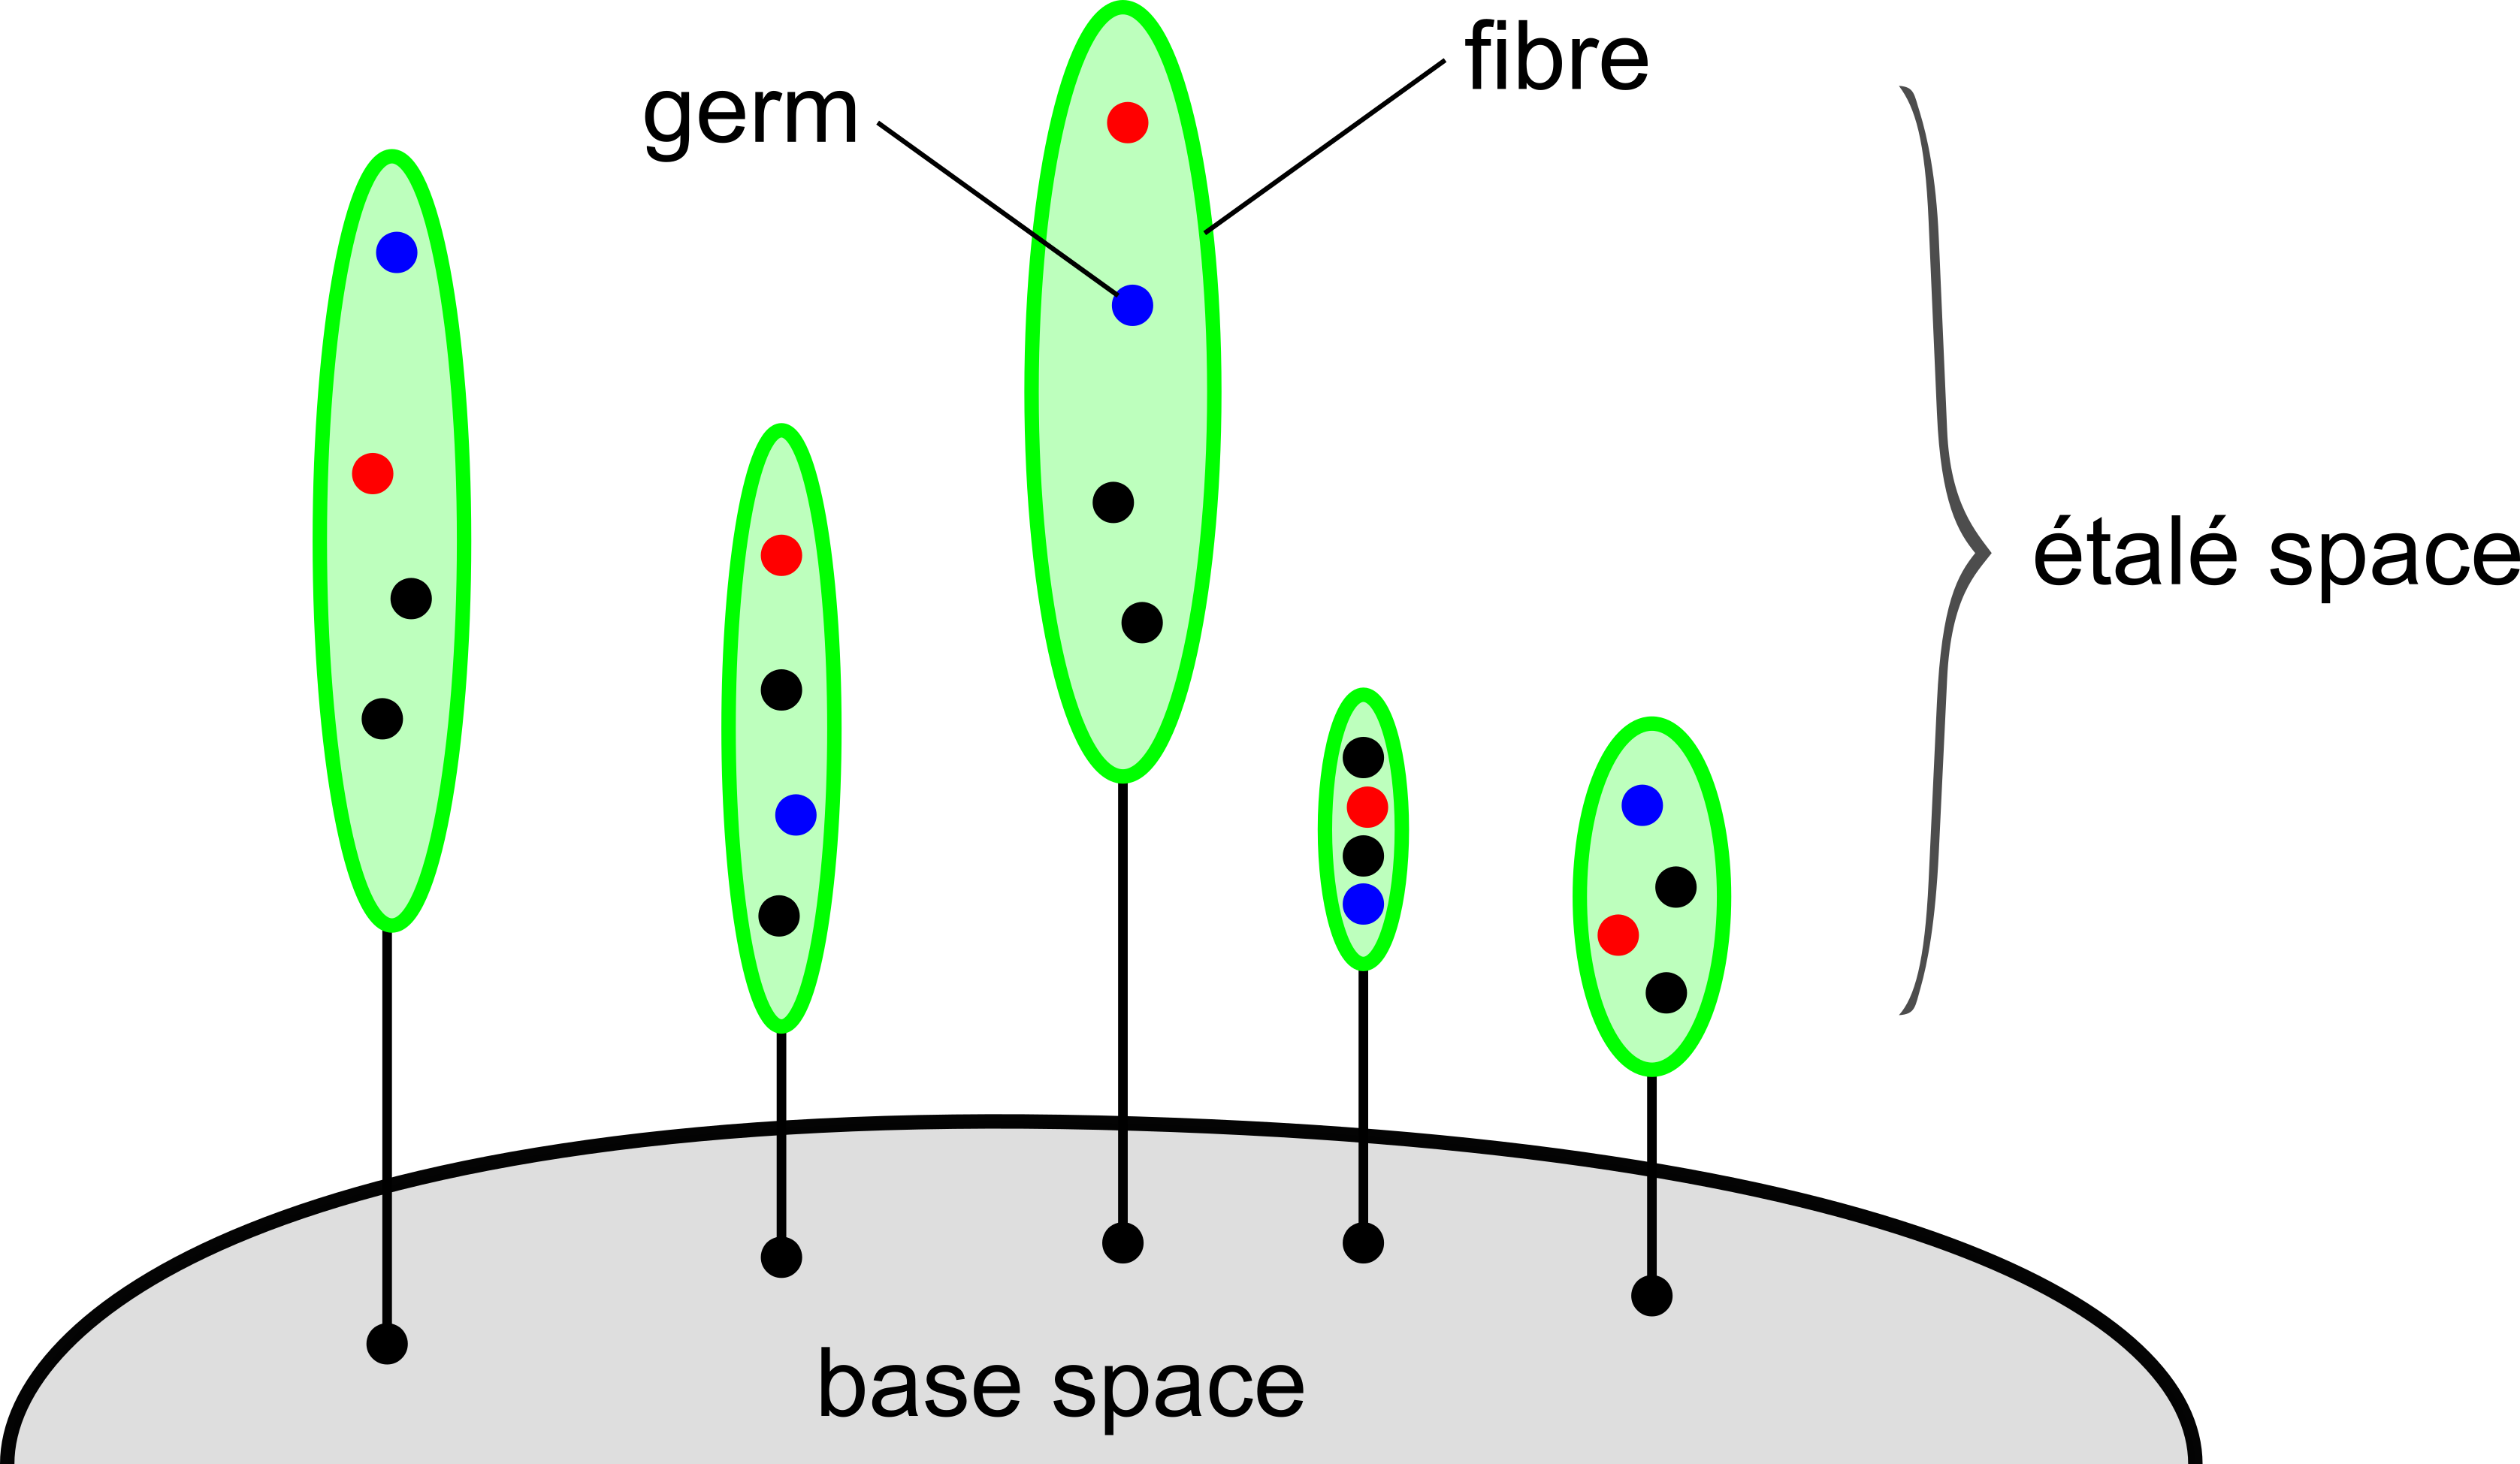
\includegraphics[scale=0.6]{etale-space.png}}}
\end{equation}

\textbf{命题逻辑} 是一种 \textbf{拓扑} (开集)结构:
\begin{equation}
\vcenter{\hbox{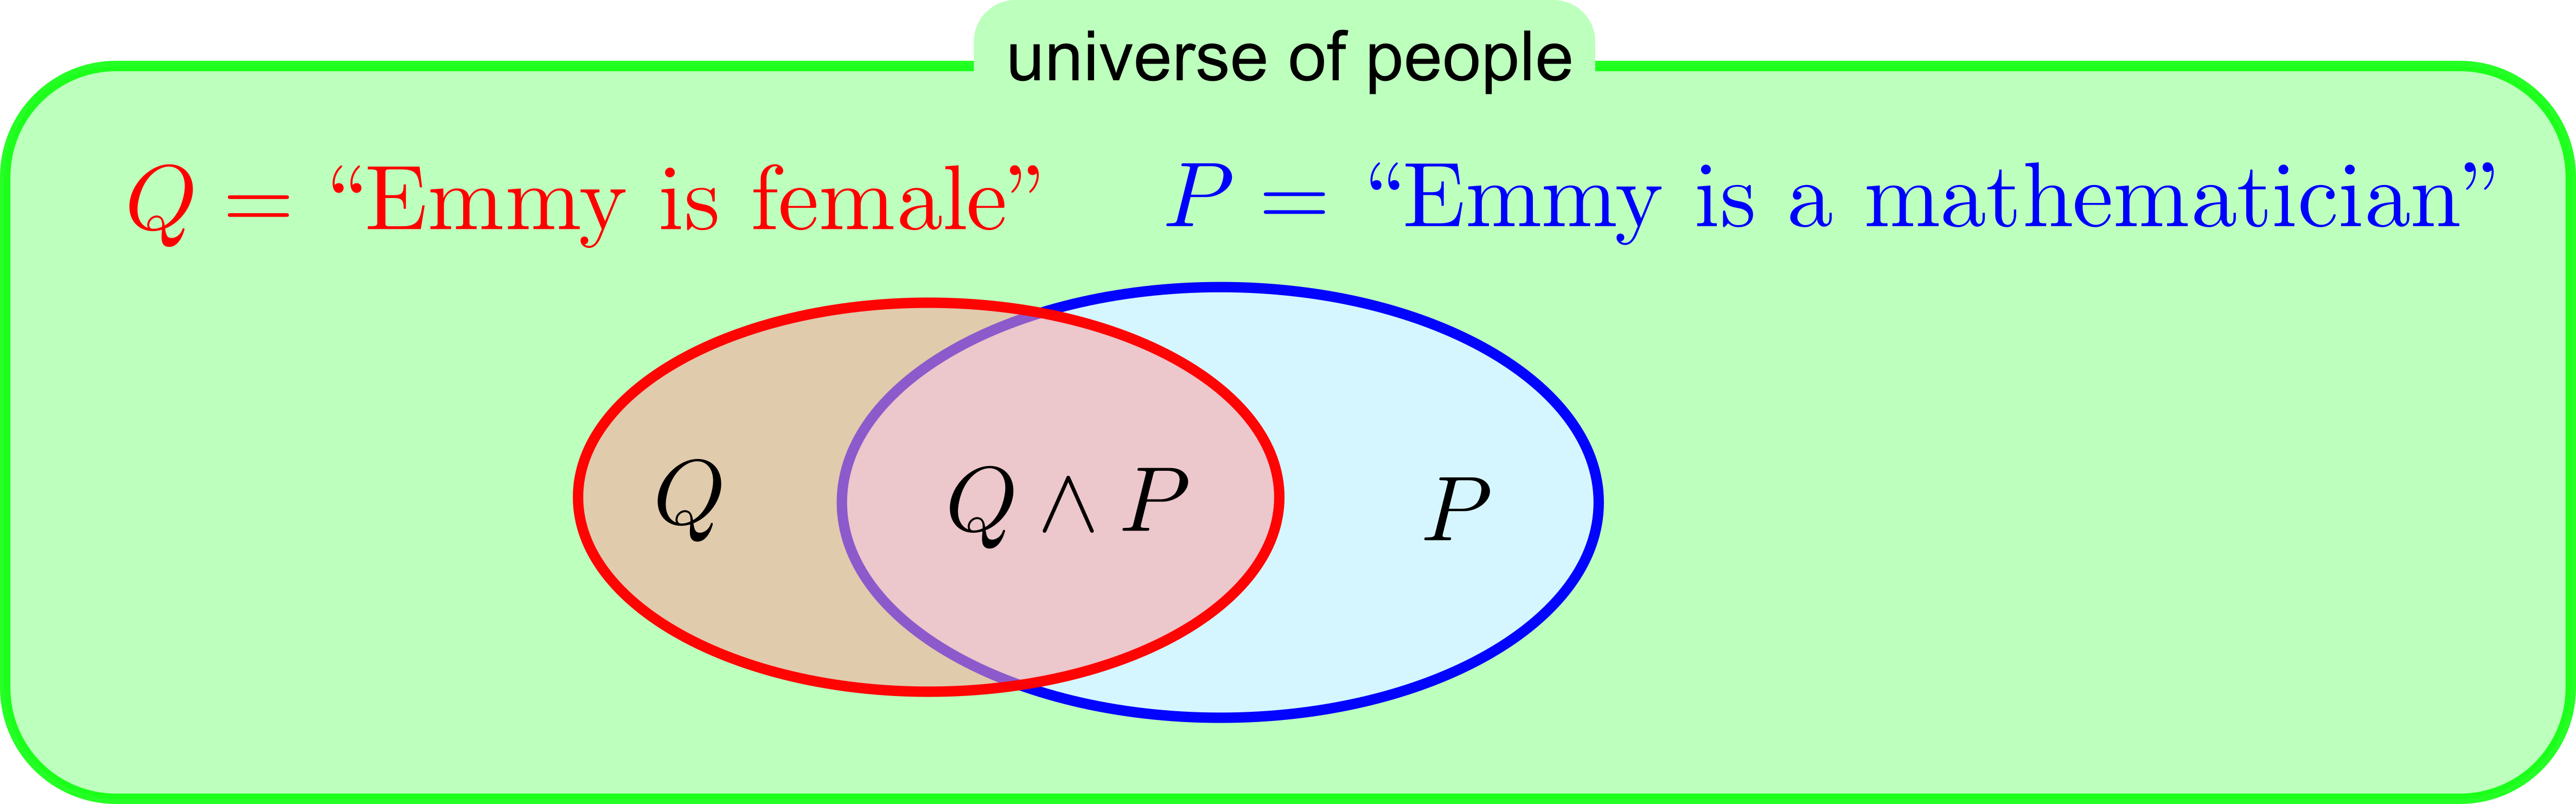
\includegraphics[scale=0.6]{propositional-logic-as-topology.png}}}
\end{equation}

如果命题的 \textbf{内部} 有结构,则变成 \textbf{谓词逻辑}:
\begin{equation}
\vcenter{\hbox{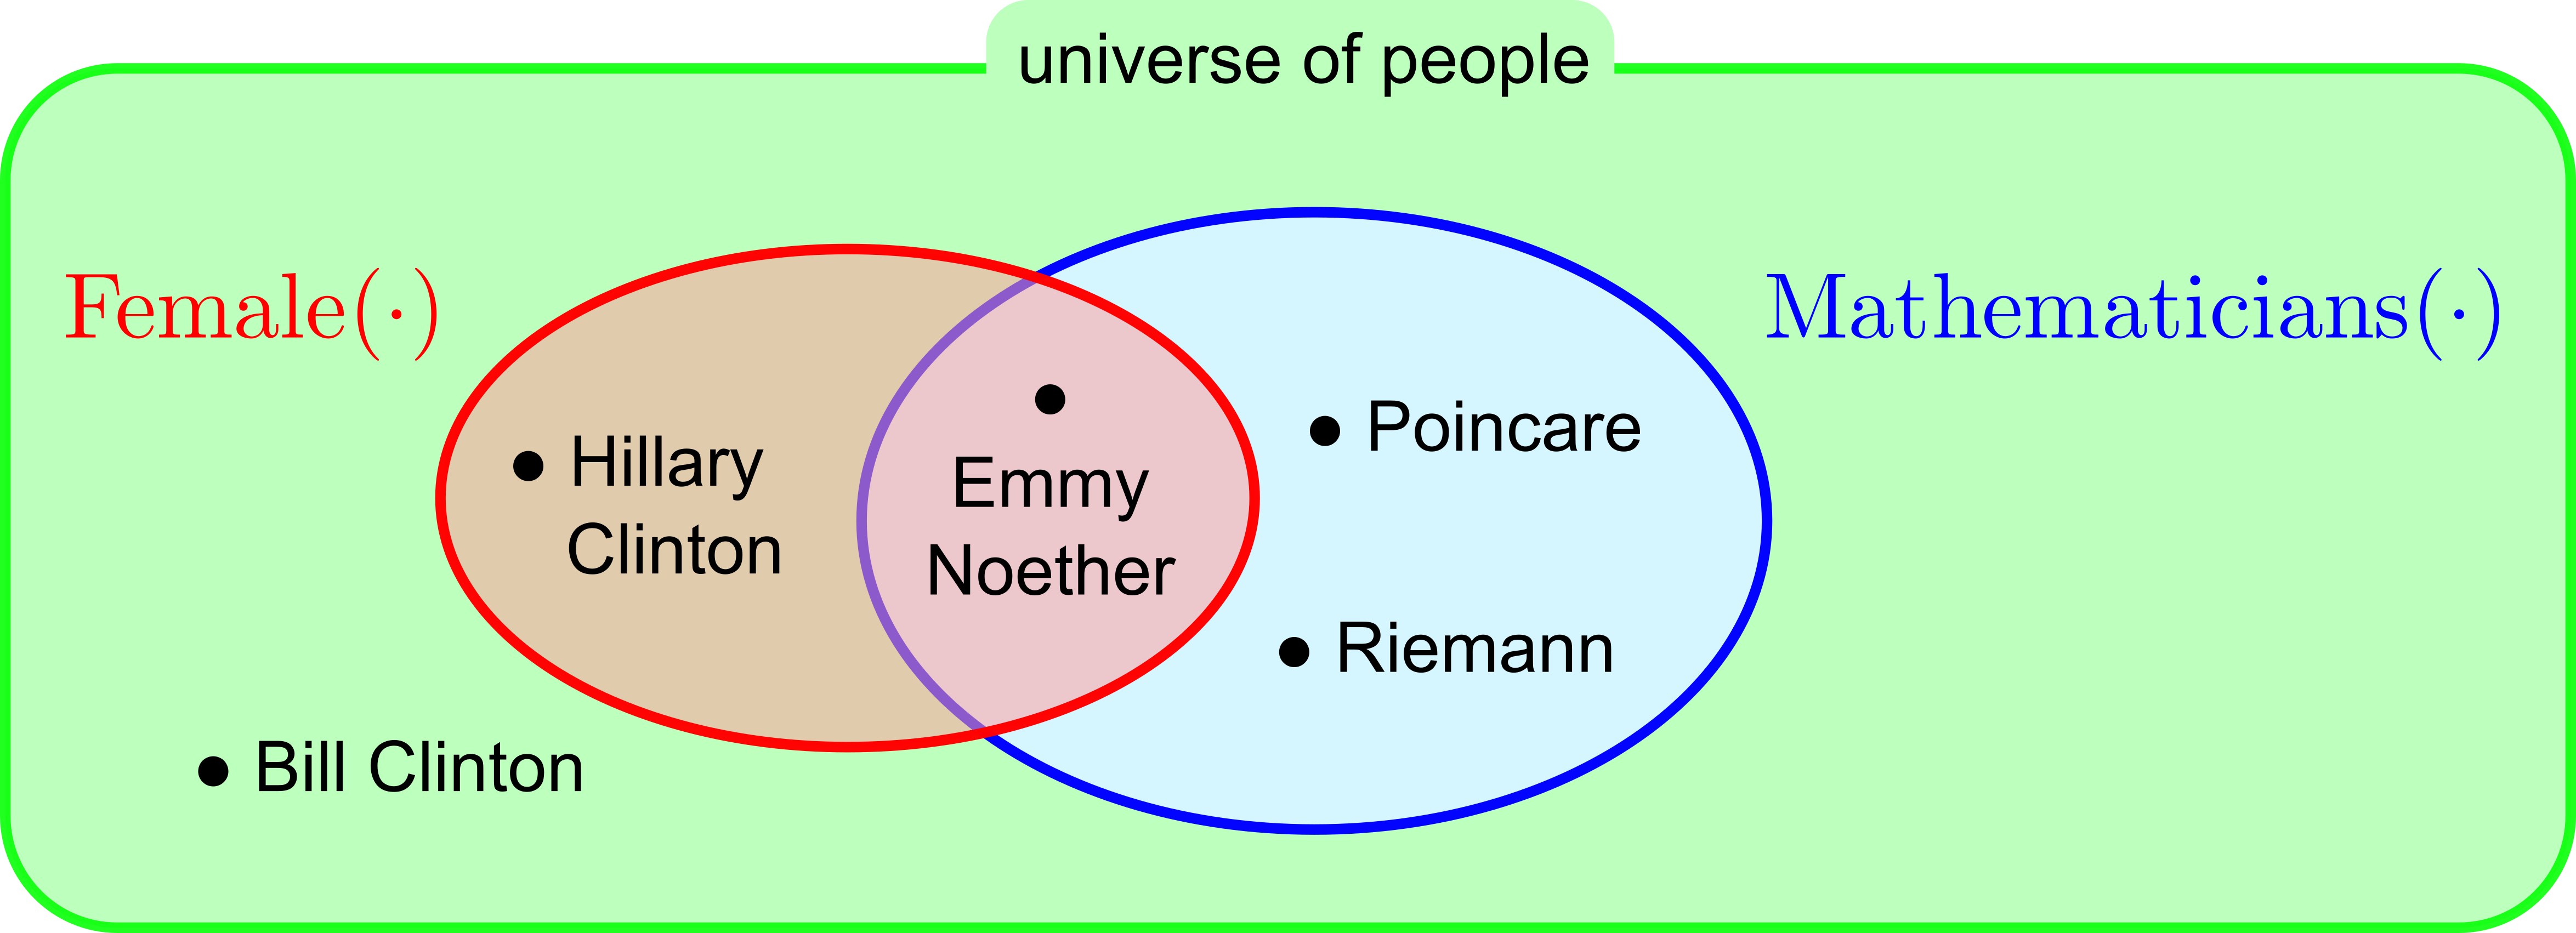
\includegraphics[scale=0.6]{predicate-logic-as-topology.png}}}
\end{equation}

谓词逻辑 可以 看作是 命题逻辑 之上的一个 \textbf{fibration}:
\begin{equation}
\vcenter{\hbox{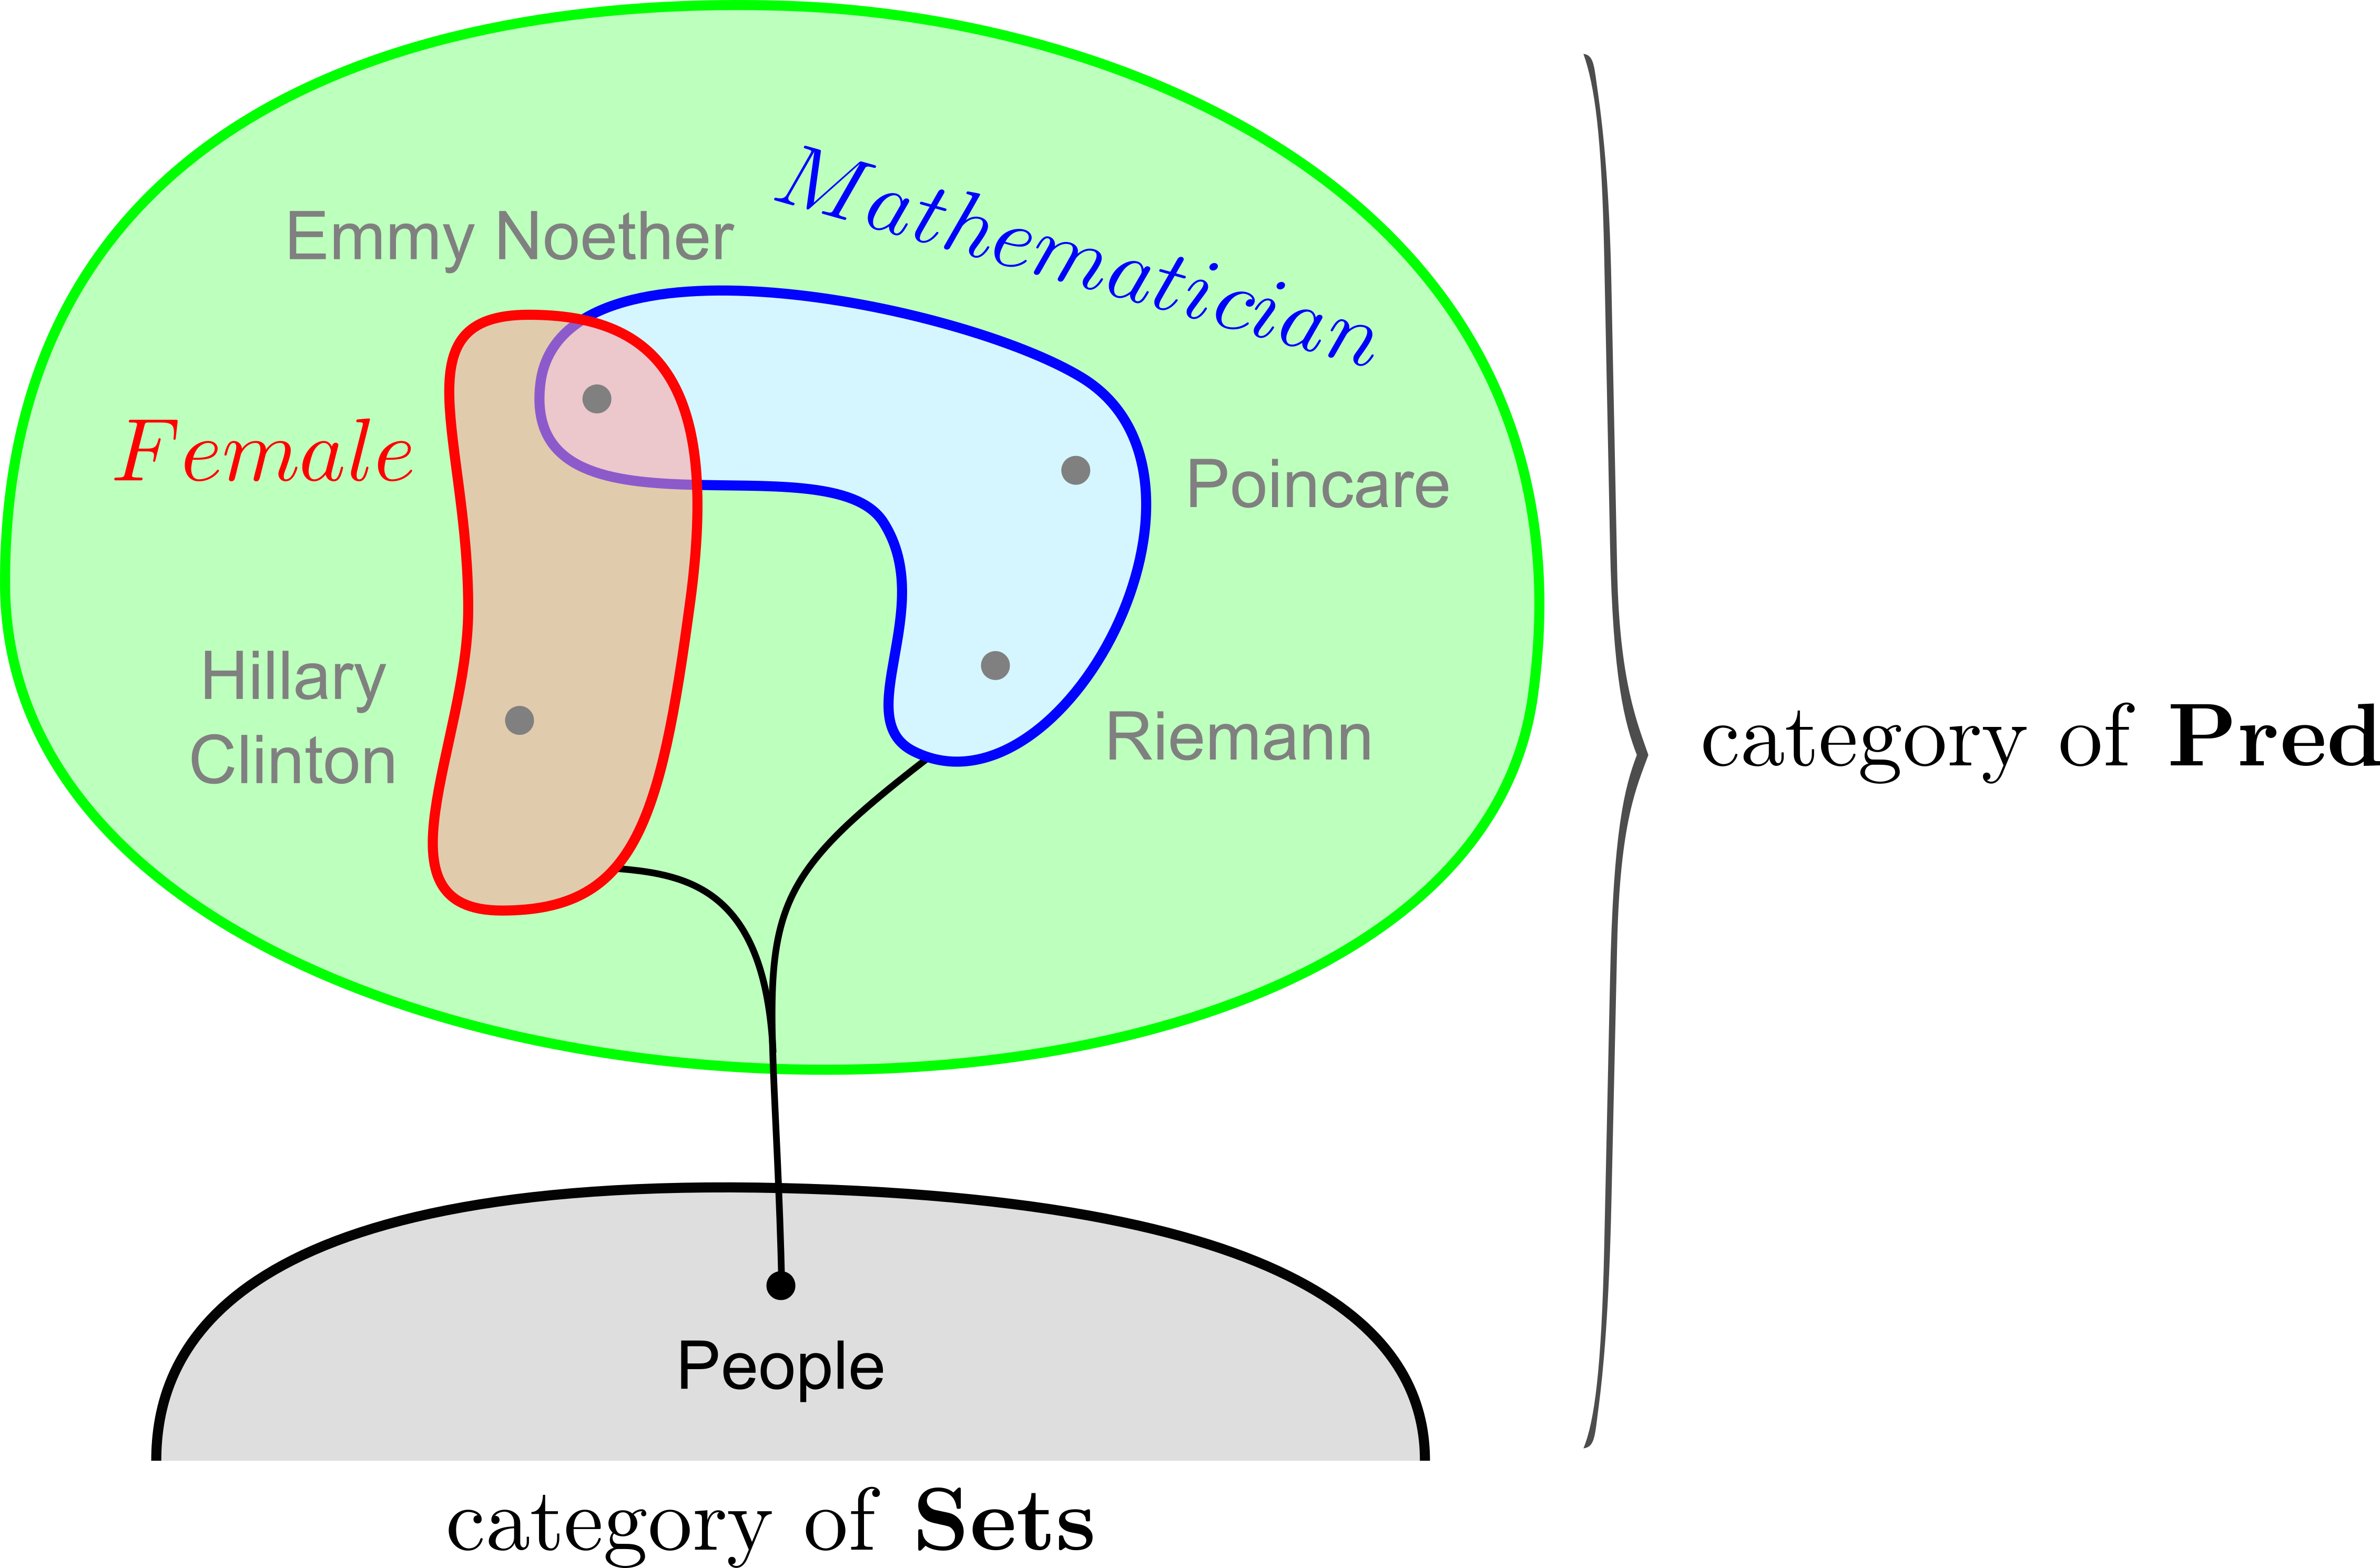
\includegraphics[scale=0.6]{predicate-logic-as-fibration.png}}}
\end{equation}
		
	
		\subsection{\cc{Lawvere 量词}{Lawvere quantification}}
		\label{sec:Lawvere-quantification}

\parencite{Lawvere1963} 提出,$\exists$ 和 $\forall$ 分别是某个 substitution map $f$ 的左和右 \textbf{adjoint} functors:
\begin{equation}
 \exists \dashv f \dashv \forall 
\end{equation}

$f$ 是一个叫 ``weakening'' 的函子,它的作用是将 论域 $X$ 扩充映射到 $X \times Y$,$Y$ 是一个新的 variable:
\begin{equation}
f: X \rightarrow X \times Y
\end{equation}
则可以定义:
\begin{eqnarray}
\exists{}_f &=& 
%\begin{tikzpicture}[overlay]
%\draw[red,fill=red] (-0.22,0.11) ellipse (5pt and 7pt);
% \draw[fill=red] (-0.4,-0.1) rectangle (-0.05,0.25);
%\end{tikzpicture}
%{}_{\exists} =
\{ y |\; \exists x.\;  \left[ y = f(x) \;\wedge\; x \in R \right] \} \nonumber \\
\forall{}_f &=&
%\begin{tikzpicture}[overlay]
%\draw[red,fill=red] (-0.24,0.11) ellipse (5pt and 7pt);
% \draw[fill=red] (-0.4,-0.1) rectangle (-0.05,0.25);
%\end{tikzpicture}
%{}_{\forall} =
\{ y |\; \forall x.\;  \left[ y = f(x) \;\rightarrow\; x \in R \right] \}
\end{eqnarray}
这里 $X$ 和 $Y$ 是任意的 \textbf{论域},而 $f: X \rightarrow Y$ 代表 论域的 \textbf{转变},
%\begin{tikzpicture}
%\draw[red,fill=red] (0,0) ellipse (5pt and 7pt);
%\end{tikzpicture} 是任意区域(子集),
所以 $f$ 是一种 ``substitution map''。

还有这两个等式 但我暂时不太理解: For all $S \subseteq X, T \subseteq Y$:
\begin{eqnarray}
& S \subseteq f^{-1} T \quad \quad \Longleftrightarrow \quad \quad \exists {}_f  S \subseteq T &\\
&\vcenter{\hbox{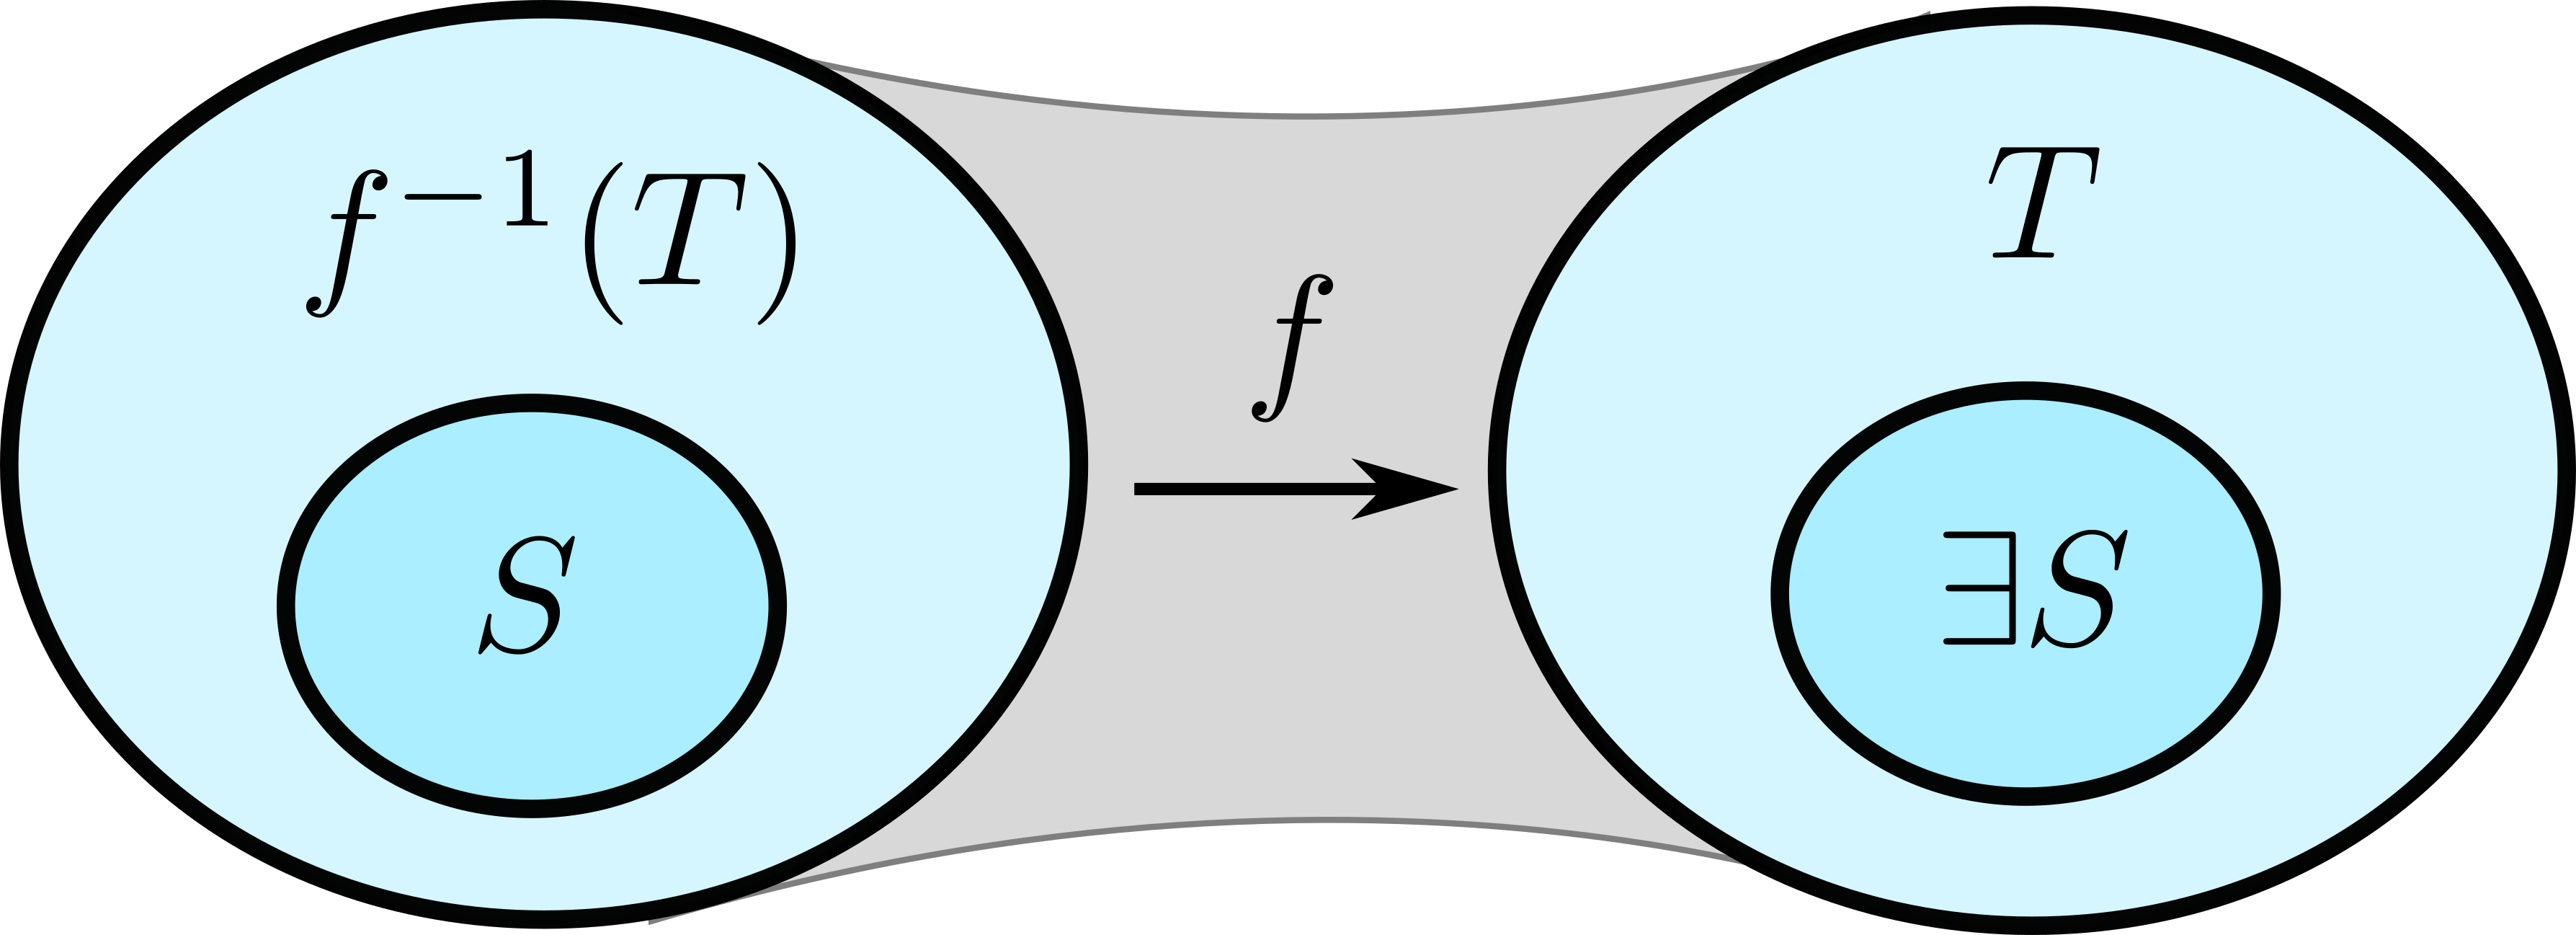
\includegraphics[scale=0.7]{Lawvere-quantifier-exists.png}}}& \nonumber
\end{eqnarray}

\begin{eqnarray}
&f^{-1} T \subseteq S \quad \quad \Longleftrightarrow \quad \quad T \subseteq \forall {}_f  S & \\
&\vcenter{\hbox{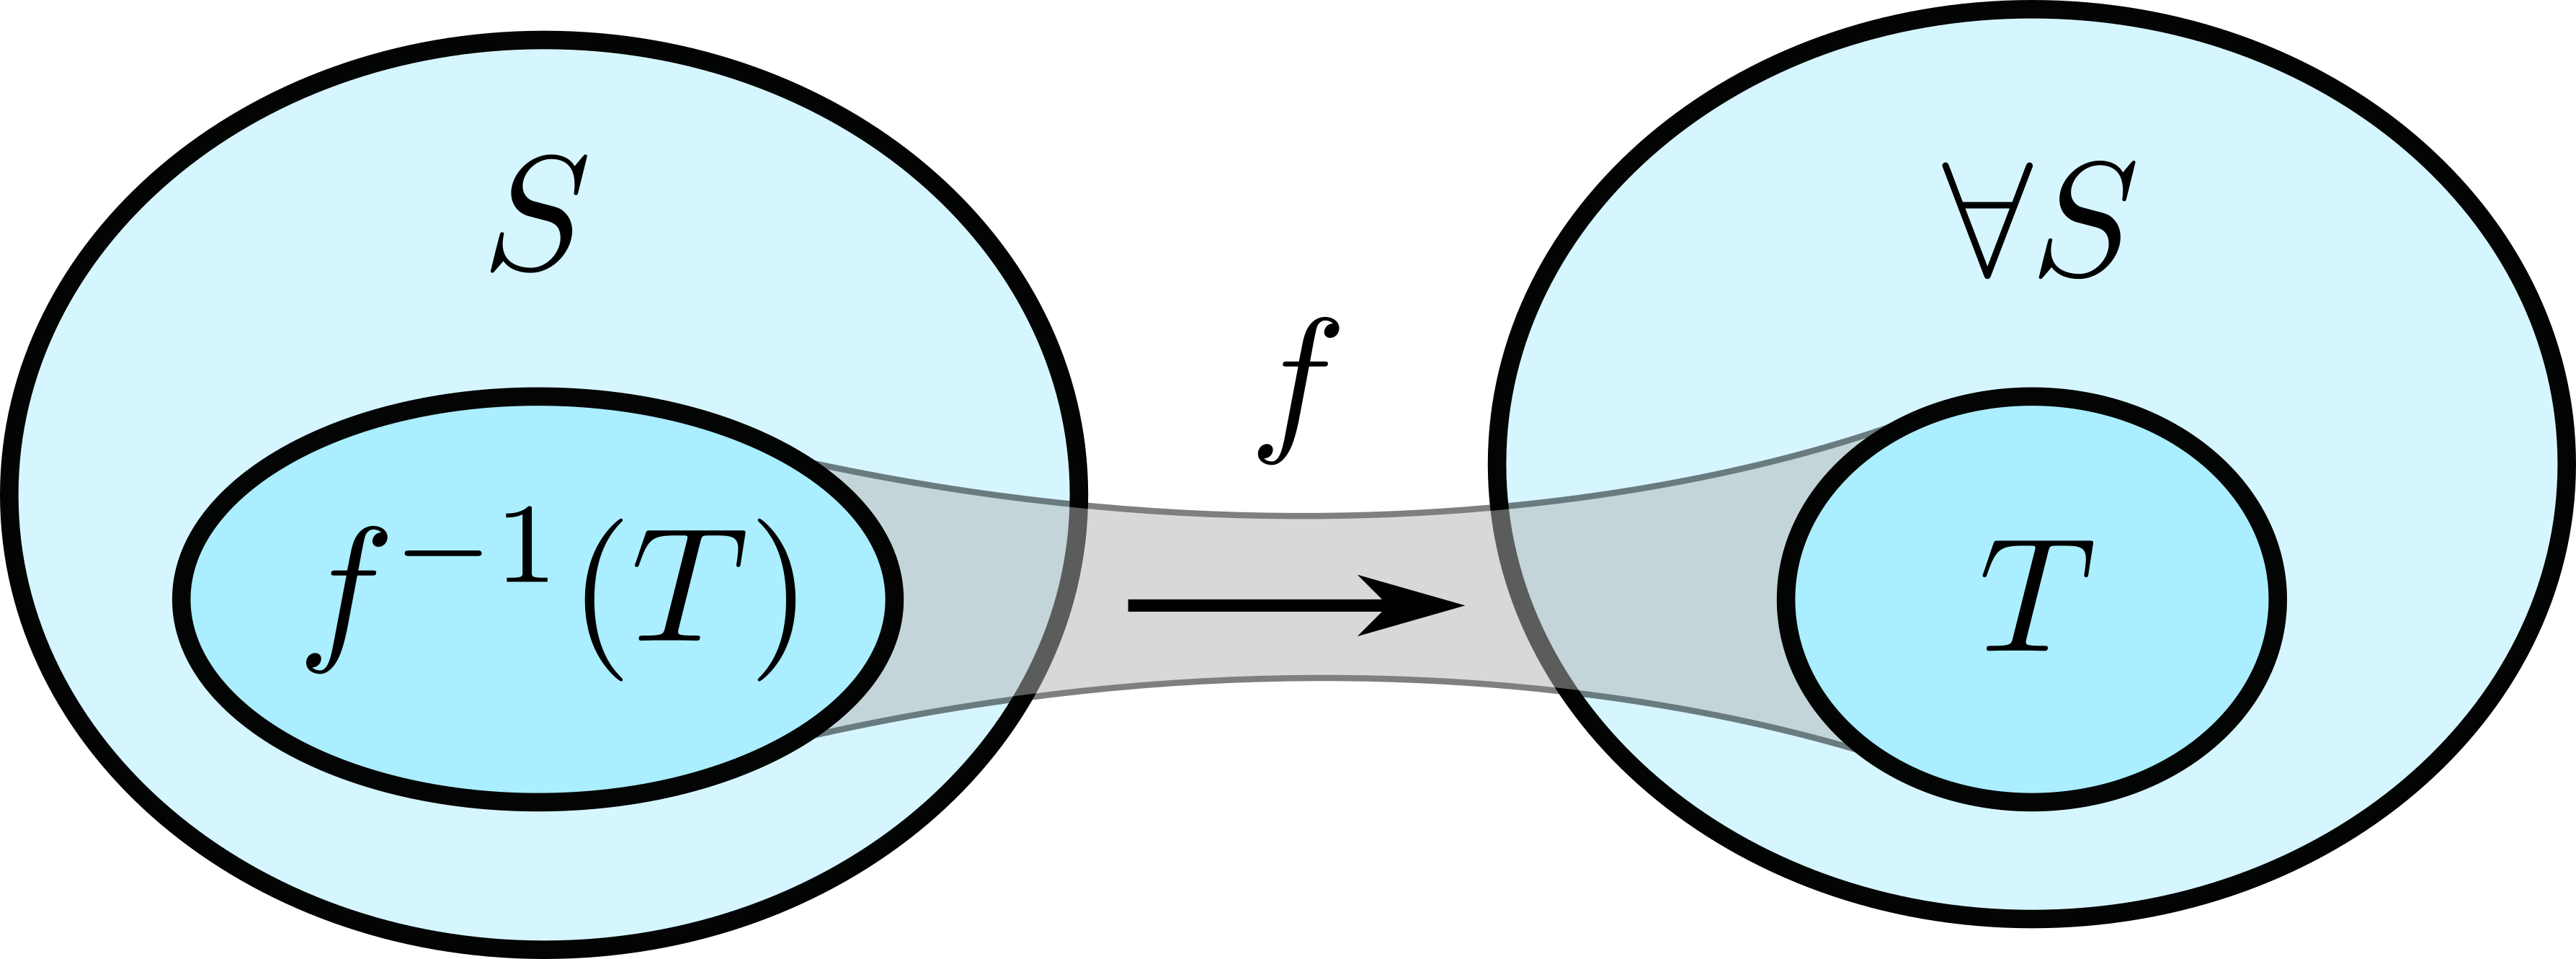
\includegraphics[scale=0.7]{Lawvere-quantifier-forall.png}}}& \nonumber
\end{eqnarray}

\parencite{Lawvere2003}, \parencite{Lawvere1963}

\subsection{Cut elimination}



	\section{\cc{量子逻辑}{Quantum logic}}
	

	
	\section{\cc{项重写系统}{Term rewriting systems}}
	
	\section{\cc{图重写系统,超图}{Graph rewriting systems, hypergraphs}}

Hypergraph 似乎和 simplicial complex 同构。

%\bibliographystyle{apalike}
%\bibliography{AGI-book}
\printbibliography[heading=secbib]
